% Thesis guidelines:
% - 40 pages including graphs, graphics and pictures, TOC/appendix/bibliography not counted
% - 1.5 line-spacing
\documentclass[12pt,a4paper,english]{article} %document type and language

\usepackage[onehalfspacing]{setspace}
% \linespread{1.5}

\usepackage[utf8]{inputenc}	% set character set to support some UTF-8
\usepackage{babel} 	% multi-language support
% \usepackage{sectsty}	% allow redefinition of section command formatting
\usepackage{tabularx}	% more table options
\usepackage{titling}	% allow redefinition of title formatting
\usepackage{imakeidx}	% create and index of words
\usepackage{xcolor}	% more color options
\usepackage{enumitem}	% more list formatting options
\usepackage{tocloft}	% redefine table of contents, new list like objects

\usepackage[centering,noheadfoot,left=3cm, right=2cm, top=2cm, bottom=2cm]{geometry}

%set TOC margins
\setlength{\cftbeforesecskip}{15pt} % skip in TOC

% remove paragraph white space and modify space between list items
\usepackage{parskip}

% Set font globally
\usepackage{lmodern}                % load Latin modern fonts
\usepackage[defaultsans]{cantarell} % cantarell fonts

% HACK: https://tex.stackexchange.com/questions/58087/how-to-remove-the-warnings-font-shape-ot1-cmss-m-n-in-size-4-not-available
\usepackage{anyfontsize}

% set LaTeX global font
\renewcommand{\familydefault}{\sfdefault}
\renewcommand{\sfdefault}{lmss}

% set styling headings
%\allsectionsfont{\usefont{OT1}{phi}{b}{n}}

\usepackage{float} 	% floats
\usepackage{graphicx}	% Graphics
\usepackage{amsmath}	% extensive math options
\usepackage{amssymb}	% special math symbols
\usepackage[Gray,squaren,thinqspace,thinspace]{SIunits} % elegant units
\usepackage{listings}                                   % source code

% Custom Operators
%% Expectation symbol
\DeclareMathOperator*{\E}{\mathbb{E}}
\DeclareMathOperator*{\Cov}{\mathrm{Cov}}
\DeclareMathOperator*{\Var}{\mathrm{Var}}

% missing math commands
\providecommand{\abs}[1]{\left\lvert#1\right\rvert}                    % |.|
\providecommand{\br}[1]{\left(#1\right)}                               % (.)
\providecommand{\sbr}[1]{\left[#1\right]}                              % [.]
\providecommand{\ddfrac}[2]{\frac{\displaystyle #1}{\displaystyle #2}}
% use \math rm{d} to include math differential

% independence symbol
% https://tex.stackexchange.com/questions/79434/double-perpendicular-symbol-for-independence
\newcommand{\indep}{\perp\!\!\!\!\perp}


% options for listings
\lstset{
  breaklines=true,
  postbreak=\raisebox{0ex}[0ex][0ex]{\ensuremath{\color{red}\hookrightarrow\space}},
  numbers=left,
  numbersep=5pt,
  numberstyle=\tiny\color{gray},
  basicstyle=\footnotesize\ttfamily
}

% NEEDS to be before hyperref, cleveref and autonum
% number figures, tables and equations within the sections
\numberwithin{equation}{section}
% \numberwithin{figure}{section}
% \numberwithin{table}{section}

% references and annotation, citations
\usepackage[small,bf,hang]{caption}        % captions
\usepackage{subcaption}                    % adds sub figure & sub caption
\usepackage{sidecap}                       % adds side captions
\usepackage{hyperref}                      % add hyperlinks to references
\usepackage[noabbrev,nameinlink]{cleveref} % better references than default~\ref
% Hack:https://tex.stackexchange.com/questions/285950/package-autonum-needs-the-obsolete-etex-package
\expandafter\def\csname ver@etex.sty\endcsname{3000/12/31}
\let\globcount\newcount
% Deactivate for now to avoid issues with equation* environment.
% \usepackage{autonum}                       % only number referenced equations
\usepackage{url}                           % URLs
% Biblatex throws error when cite is used.
% Similar warning is given by natbib.
% \usepackage{cite}                          % well formed numeric citations

% % biblatex for references
% \usepackage{biblatex}
% \addbibresource{literature.bib}
% % csquotes recommended: https://tex.stackexchange.com/questions/229638/package-biblatex-warning-babel-polyglossia-detected-but-csquotes-missing
% \usepackage{csquotes}
% \addbibresource{refs.bib}

% https://tex.stackexchange.com/questions/144764/author-year-citation-in-latex
\usepackage[round]{natbib}

% Avoid space before footnotes when \footnote{...} is on next line.
% https://tex.stackexchange.com/questions/94563/new-line-for-footnote-without-blank-space
\usepackage{xpatch}
\xpretocmd{\footnote}{\unskip}{}{}

% format hyperlinks
\colorlet{linkcolour}{black}
\colorlet{urlcolour}{blue}
\hypersetup{colorlinks=true,
            linkcolor=linkcolour,
            citecolor=linkcolour,
            urlcolor=urlcolour}

%\usepackage{todonotes} % add to do notes
\usepackage{epstopdf}  % process eps-images
\usepackage{float}     % floats
\usepackage{fancyhdr}  % header and footer
% HACK: https://tex.stackexchange.com/questions/664532/fancyhr-warning-footskip-is-too-small
\setlength{\footskip}{15pt}

% default path for figures
\graphicspath{{figures/}}

% If we have multiple directories, specify them like this: \graphicspath{{figures_ch1/}{figures_ch2/}}.

% For rendering tikz
\usepackage{pgfplots}
\pgfplotsset{compat=1.18}
\usetikzlibrary{decorations.pathreplacing} % Load the library for drawing braces


% Define some math environments
\usepackage{amsthm}

\newtheorem{theorem}{Theorem}[section]
\newtheorem{corollary}{Corollary}[theorem]
\newtheorem{lemma}[theorem]{Lemma}

\theoremstyle{definition}
\newtheorem{definition}{Definition}[section]

\theoremstyle{remark}
\newtheorem*{remark}{Remark}

\theoremstyle{plain}
\newtheorem{assumption}{Assumption}

% https://tex.stackexchange.com/questions/24840/use-courier-font-inline-on-text
\usepackage{courier}

% https://tex.stackexchange.com/questions/639234/how-to-put-braces-over-certain-parts-of-matrices
\usepackage{nicematrix}


% set header and footer
\pagestyle{fancy}
\fancyhf{}                           % clear all header and footer fields
\cfoot{\thepage}                     % add page number
\renewcommand{\headrulewidth}{0pt} % add horizontal line of 0.4pt thick

\title{Statistical Inference in Partially Identified Marginal Treatment Effect Models}
\author{Julian Budde}
\date{\today}
\begin{document}

\maketitle

\begin{abstract}
	I study inference in the marginal treatment effect model when used to partially-identify a target parameter of interest.
	First, I demonstrate the invalidity of the nonparametric bootstrap in a simple, but common binary IV model.
	In specific settings, the bounds of the identified set have an easy to calculate solution.
	These solutions exhibit points of non-differentiability when viewed as functions of the point-identified parameters hence rendering the nonparametric bootstrap invalid.
	Similar issues arise when a parametric approximation to the MTR functions is used.
  Second, I discuss potential solutions proposed in the literature and show how they might be adjusted to typical use-cases where bounds have to be calculated by the means of linear programming.
	Third, for a number of empirically relevant settings I conduct novel simulation studies for the MTE model comparing competing inference methods.
  Lastly, I suggest a conservative inference approach to the value of a linear program by a strict convex relaxation of the constraint set.
  I illustrate the performance of this method in a simple Monte Carlo experiment.
\end{abstract}

\clearpage
\newpage

\tableofcontents

\clearpage
\newpage

\listoftables

\clearpage
\newpage

\listoffigures

\clearpage
\newpage

\section{Introduction}\label{sec:introduction}

\section{Bootstrap Invalidity: A Simple Example}\label{sec:simple_example}
I first illustrate the invalidity of the bootstrap in a simple example with a binary instrument where we only use the point-identified LATE for the instrument-compliers as the basis for extrapolation.
While this will not best we can do in this case --- there are more moments in the data we can point-identify --- it helps to illustrate the type of inference issues that can also arise in more complex setups.
In particular, we can calculate explicit solutions for the upper and lower viewed as functions of the point-identified complier LATE.\@

\subsection{Setup}
We first introduce some basic notation and key ingredients of the MTE model.
A complete statement of the model corresponding to~\cite{mogstad2018using} can be found in Section~\ref{sec:general_mte}.

The outcome is denoted $Y_i$ and has bounded support, which we generally assume to be in $[0,1]$ for convenience.
The instrument $Z_i$ is binary with realizations in $\{0,1\}$.
Binary treatment $D_i$ is determined by a selection model with
\begin{equation}\label{eq:treatment}
  D_i = I\{p(Z_i) \geq U_i\}
\end{equation}
where unobserved heterogeneity $U_i$ is normalized to follow a $U(0,1)$ distribution, $U_i \indep Z_i$ and $I\{A\}$ denotes the indicator function for event $A$.
Hence, $p(z) \equiv P(D_i=1|Z_i=z)$ is the propensity score. We define the instrument $Z_i$ such that $p(0)<p(1)$.

As shown by~\cite{vytlacil2002independence}, under an appropriate set of assumptions stated more formally in Section~\ref{sec:general_mte}, this setup is equivalent to the potential outcome framework in~\cite{imbens_angrist1994ecma}.
Hence, we can point-identify a local average treatment effect for the instrument-compliers, namely those individuals, who take up the treatment if and only if $Z_i=1$.
In the selection model above, the complier subpopulation is those with $U_i$ realizations in $[p(0), p(1)]$.
Hence, in the notation of the model, we can point-identify,
\begin{equation}
  \beta_s = \E[Y(1) - Y(0)|U_i\in[p(0), p(1)]].
\end{equation}
Note that individuals with realizations $u \leq p(0)$ will always select into treatment, while individuals with $u \geq p(1)$ will never select into treatment.
To keep the notation light, I will refer to these subpopulations as \textit{complier}, \textit{never-taker} and \textit{always-taker}.

Our goal is to extrapolate from this identified complier-LATE to a larger subpopulation that also includes some never-takers.
[Example for interpretation]. Now we are interested in a policy-change which we would believe to increase the propensity score.
We denote this new target by
\begin{equation}
  \beta^* = \E[Y(1) - Y(0)|U_i \in[p(0), p(1) + \overline{u}]],
\end{equation}
where $\overline{u}\in[0, 1-p(1)]$.

Without very strong restrictions, $\beta^*$ will not be point-identified.
Instead, we will only generally be able to identify a set of values for the target that are both consistent with the data and theoretical assumptions we want to impose.
Usually, this \textit{identified set} will be a closed interval on the real line, and we will denote it by
\begin{equation*}
  \beta^* \in [\underline{\beta^*}(\beta_s), \overline{\beta^*}(\beta_s)],
\end{equation*}
where we emphasize the dependence of the upper and lower bound of the identified set on the point-identified parameter $\beta_s$.

\subsection{Solution: Nonparametric Bounds}
While the identified set is usually computed via a linear program, in the simple case considered here with a single point-identified parameter the identified set has an intuitive and easy to compute form.
Note the following solutions are referred to as \textit{nonparametric} in~\cite{mogstad2018using}, that is, they do not impose any parametric assumptions on the underlying MTR functions.
The corresponding linear program solution can be achieved by using constant splines defined on the grid $[0, p(0), p(1), p(1) + \overline{u}, 1]$.

Denote by $\beta_{\overline{u}}$ the LATE for the population of never-takers for which we want to extend the treatment, i.e.
\begin{equation*}
  \beta_{\overline{u}} \equiv E[Y(1) - Y(0) | u \in [p(1), p(1) + \overline{u}]].
\end{equation*}
Then $\beta^*$ is a weighted average of the two LATEs:\@
\begin{equation*}
  \beta^* = \omega\beta_s + (1-\omega)\beta_{\overline{u}}
\end{equation*}
where $\omega = \frac{p(1) - p(0)}{\overline{u} + p(1) - p(0)}$ is the relative share of compliers in the target population.
Finding the identified set then amounts to finding bounds on $\beta_{\overline{u}}$, where different restrictions imply different bounds.



\paragraph{Nonparametric Bounds}
Without any further restrictions, the only bounds we can give follow from the support of $Y_i$.
Since $Y_i\in[0,1]$ we have $\beta_{\overline{u}} \in [0,1]$ and hence
\begin{equation*}
  \beta^* \in [\omega\beta_s - (1 - \omega), \omega\beta_s + (1 - \omega)]
\end{equation*}
We can already see that this is a continuous and differentiable function of $\beta_s$.
Hence, if estimation for $\beta_s$ and $\omega$ is standard, the usual delta method could be applied.
This is the case here, since $\beta_s$ can be consistently estimated using the Wald estimator which --- assuming no weak identification issues --- is asymptotically normal.
$\omega$ is a function of sample moments and can be estimated consistently.
Therefore, also the nonparametric bootstrap is valid in this case.
\footnote{The only issue would arise at the boundary of the parameter space, that is when $\underline{\beta^*}(\beta_s)=-1$ or $\overline{\beta^*}(\beta_s)=1$.
These cases are of less interest practically, hence I disregard them. However, a similar issue arises under shape restrictions discussed below.}

\paragraph{Monotone Marginal Treatment Effect}
We can impose the assumption, that the treatment effects $E[Y(1) - Y(0)|U_i=u]$ are monotone in $u$.
In the language of~\cite{mogstad2018using}, the MTE function is monotone.
The most interesting assumption is a \textit{decreasing} MTE function, since treatment take-up is decreasing in $u$.

If the MTE function is decreasing, we know $\beta_{\overline{u}} \leq \beta_s$ and hence the identified set shrinks at the upper bound:
\begin{equation*}
  \beta^* \in [\omega\beta_s - (1 - \omega), \beta_s]
\end{equation*}
In this case, inference is again standard. Note we have point identification when $\beta_s=-1$.
\footnote{Convergence to point-identification can pose problems to the type of confidence intervals considered by~\cite{imbens2004confidence} and considered later here.
In particular, coverage does not hold uniformly over parameter sequence implying convergence to point-identification.
~\cite{imbens2004confidence} propose a simple adjustment that I discuss in more detail in Section~\ref{sec:simulation_studies}.}


\paragraph{Monotone Treatment Response}
Under monotone treatment response, it is assumed that all individuals respond either negative or positive to the treatment.
An implication for the marginal treatment effect is that it is either positive or negative everywhere.
This again tightens the set, but it also restricts the parameter space of $\beta_s$ that is consistent with the model.
In particular, any $\beta_s \leq 0$ is inconsistent with the assumption of positive treatment responses.
In addition, the lower bound will be tighter:
\begin{equation*}
  \beta^* \in \begin{cases}
    [\omega\beta_s, \beta_s + (1 - \omega)] & \beta_s \geq 0 \\
    \emptyset & \beta_s < 0
  \end{cases}
\end{equation*}
Here, inference becomes non-standard at the boundary of the parameter space.
This case is close to the stylized example analyzed in~\cite{andrews1999estimation}, where interest lies in estimating an expectation which is known to be positive.
[Explain, why not focusing on this in the following.]

\paragraph{Decreasing Marginal Treatment Responses}
A last restriction considered by~\cite{mogstad2018using} are monotonicity restrictions on the MTR functions $m_d(u) = E[Y(d)|U=u]$.
We consider the case of increasing MTR functions.
Imposing restrictions on these functions is also the general approach discussed in Section~\ref{sec:general_mte}, since this allows to exploit other moments for identification.
For example, in our model also $E[Y(1)|\text{always-taker}]$ and $E[Y(0)|\text{never-taker}]$ are identified and can help in tightening the identified set.

While generally not impossible, with the restriction that $m_0(u), m_1(u)$ are increasing in $u$, the computation of the identified set becomes less immediate.
% Figure [TODO REF] illustrates the solution using constant spline basic functions defined separately over the intervals implied by $[0, p(0), p(1), p(1) + \overline{u}, 1]$.
Essentially, since both the identified and target parameter are averages over the MTR (or MTE) function with constant weights on each sub-interval, taking constant splines on these sub-intervals as basis functions does not impose any additional restrictions.

The solution in this case is given by:
\begin{equation}\label{eq:solution_cs_increasing_mtr_upper}
	\overline{\beta^*}(\beta_s)=
	\begin{cases}
		\omega \beta_s + (1 - \omega),& \quad \text{if } \beta_s \geq 0\\
		\beta_s + (1 - \omega),              & \quad \text{if } \beta_s < 0,
	\end{cases}
\end{equation}
and
\begin{equation}\label{eq:solution_cs_increasing_mtr_lower}
	\underline{\beta^*}(\beta_s)=
	\begin{cases}
		\beta_s - (1 - \omega),& \quad \text{if } \beta_s \geq 0\\
		\omega \beta_s - (1 - \omega),              & \quad \text{if } \beta_s < 0.
	\end{cases}
\end{equation}

Hence, both bounds exhibit a kink at $\beta_s=0$.
In these cases, as was shown in~\cite{dumbgen1993nondifferentiable} and later~\cite{fang2019infdirdiff}, non-differentiability at the kink renders the nonparametric bootstrap invalid.
However, other methods have been devised for this case. For example,~\cite{fang2019infdirdiff} and~\cite{hong2018numerical} extend the delta method to the case of functions that are only directionally differentiable, such as the ones with a kink shown above.
Further, subsampling is theoretically justified as long as the bounds of the identified set have \textit{any} limiting distribution.
I consider these methods as well as the nonparametric bootstrap in more detail in Section~\ref{sec:inference_methods} and provide simulation evidence in a realistic setting in Section~\ref{sec:simulation_studies}.

\subsection{Solution: Bounds with Bernstein Polynomials}
In most applications, the nonparametric identified set resulting from constant splines will feature solutions, i.e. MTR functions, that exhibit jump discontinuities.
[Maybe put a solution in the appendix similar to Bernstein figures?].
The appeal of the MST framework is, that the MTR functions have direct economic interpretations that allow to place theoretical restrictions about which meaningful discussions are possible.
In particular, in most cases a certain degree of smoothness in these functions seems reasonable.

To implement this in a tractable manner,~\cite{mogstad2018using} propose to use Bernstein polynomials as basis polynomials for the MTR functions, because they exhibit many computational advantages.
For example, shape restrictions, including monotonicity of the MTR or MTE functions as well as monotone treatment response, can be easily implemented in a linear program.
\footnote{For details on the implementation of shape restrictions see Appendix Section~\ref{app_sec:linear_programs}.}

The Bernstein polynomial of degree $k$ is given by the sum over $k+1$ basis polynomials:
\begin{equation*}
  B_k(x) := \sum_{v=0}^n c_v b_{v,n}(x) \qquad \text{ where } b_{v,n}(x) := \binom{n}{v} x^v(1-x)^{n-v}, \qquad v = 0, \ldots, k.
\end{equation*}

For example, for $k=2$, we have
\begin{equation*}
  B_2(x) = c_0 (1-x)^2 + c_1 2x(1-x) + c_2 x^2.
\end{equation*}

Using these basis polynomials, it is easy to construct a linear program such that the implied MTR functions are smooth over $[0,1]$ and have images in $[0,1]$ (or any other interval, for that matter).
However, the value function of the linear program, that is the upper or lower bound of the identified set, can still be \textit{non-smooth} and feature kinks.

To illustrate, I return to the binary-IV example discussed above for nonparametric bounds.
Because the analytical solution is non-trivial to characterize for polynomials of degree $\geq2$, I instead repeatedly solve the linear program over a range of parameter values for the compliers LATE $\beta_s$.
\footnote{For a precise statement of the problem see Section~\ref{sec:general_mte} and Appendix Section~\ref{app_sec:linear_programs} for the linear program.}
I report results for a lower-order, meaning more restrictive, polynomial of degree $2$ as well as a $11$th order polynomial similar to the numerical example in~\cite{mogstad2018using}.
\footnote{
  To construct the solutions, I first use DGPs with a constant spline MTR function defined on the sub-intervals of $[0, p(0), p(1), p(1) + \overline{u}, 1]$.
  To vary $\beta_s$ I change the coefficients on the constant spline on the complier sub-interval $[p(0), p(1)]$.
  While in principle this DGP is inconsistent with a Bernstein polynomial used in identification,
  note that the MTR functions are only used to compute $\beta_s$ and play no role otherwise.
}

Figure~\ref{fig:id_set_binary_iv_bernstein} plots the solution to the lower bound $\underline{\beta}^*(\beta_s)$ as a function of the identified late.
In addition to the lower bound, the figure also shows the basis function coefficients that solve the linear program separately for $m_0$ and $m_1$.
The corresponding solution for the upper bound is symmetric, since no other shape restrictions are placed on the problem. Hence, I focus on the lower bound only for clarity.

Notably, while still continuous, these solutions again exhibit kinks, this time even without any shape restrictions.
While also visually notable, I estimate the position of the kinks by checking for discontinuities in estimated second derivatives.
These positions are indicated by gray lines and align well with the visual kinks.
From the lower subplots it is easy to see, that the kinks are associated with corner solutions of the linear programs, where coefficients start to increase from 0 or decrease from 1.
This feature is present for both reported degrees, $k=3$ and $k=11$.

Notably, increasing the degree of the polynomial has three effects:
First, as expected, the lower bounds become smaller, since the space of possible solutions is larger.
Second, the solution exhibits more kinks. In fact, the number of kinks equals the number of basis polynomials.
Lastly, increasing the number of polynomials sharply increases the slope of the solution close to 1, that is the boundary of the parameter space.
If we think of an increasing sequence $k$, this could indicate a failure of Lipschitz continuity close to the boundary.

\begin{figure}

  \caption{Identified Sets for the Binary-IV Model with Bernstein Polynomial MTRs}\label{fig:id_set_binary_iv_bernstein}

  \centering
  \begin{subfigure}[b]{0.49\textwidth}
      \centering
      \includegraphics[width=\textwidth]{../../bld/figures/binary_iv/id_bernstein_2_none_late.png}
      \caption{Degree $k=2$}\label{fig:id_set_binary_iv_bernstein_k_2}
  \end{subfigure}
  \hfill
  \begin{subfigure}[b]{0.49\textwidth}
      \centering
      \includegraphics[width=\textwidth]{../../bld/figures/binary_iv/id_bernstein_11_none_late.png}
      \caption{Degree $k=11$}\label{fig:id_set_binary_iv_bernstein_k_11}
  \end{subfigure}
\end{figure}

\paragraph{Shape Constraints}
When adding shape constraints, the qualitative features of the solution that can pose problems for inference do not change.
[Construct Appendix Figures under shape constraints.]
However, adding further shape constraints typically reduces the solution space and hence can increase

To summarize, in this section I considered a simple binary IV model which already exhibits some problems for inference in the MTE model:
First, many solutions to the MTE problem exhibit \textit{kinks} when viewed as a function of the point-identified parameters.
Kinks are present under certain shape restrictions for the nonparametric identified set using constant splines and are a general feature when using Bernstein polynomials.
Non-differentiability generally renders typical inference approaches like the nonparametric bootstrap inconsistent, as observed by~\cite{dumbgen1993nondifferentiable}.
Second, for Bernstein polynomials, the slope of the solutions close to the boundary of the parameter space exhibits increasing slopes over the degree $k$.
This could potentially indicate a failure of Lipschitz continuity.
Lastly, introducing shape restrictions, in particular monotonicity and sign constraints on the implied MTE function $m_1(u) - m_0(u)$, can significantly reduce the parameter space consistent with the model.
This can lead to parameter at the boundary issues, as, for example, discussed in~\cite{andrews1999estimation}.

\subsection{Simulation: Bootstrap and Adjusted Delta Methods}
This section presents some simple Monte Carlo evidence on the failure of the nonparametric bootstrap in the case of constant splines (``nonparametric'' bounds) with the restriction of increasing MTR functions.
\footnote{All simulations in the present paper where performed on the Marvin High-Performance-Computing Cluster at the University of Bonn.}
I take the target $LATE(0.4, 0.8)$ and a binary instrument $Z$ with propensity scores $p(0) = 0.4 < 0.6 = p(1)$ and $P(Z=0)=P(Z=1)=0.5$.
The outcome data is generated as $Y(d) = \gamma_d^g + \varepsilon$ where $\varepsilon \sim N(0,\sigma^2)$ with $\sigma=0.1$ and $g=g(u)$ refers to the three subpopulations (complier, never-taker, always-taker).
We treat only the complier late $\gamma_1^c - \gamma_0^c$ as point-identified and the remaining parameters are chosen such that the true parameter is at the upper bound of the identified set.

I construct confidence intervals by estimating the quantiles of the asymptotic distribution of the estimated upper bound denoted by
\begin{equation}
  \sqrt{N}(\hat{\overline{\beta}^*} - \overline{\beta}^*) \to_d \overline{G},
\end{equation}
where $\overline{\beta}^*$ is the sample analogue of Equation~\ref{eq:solution_cs_increasing_mtr_upper}, and analogously for the lower bound.
In the current case, given the closed form solution it is easy to show using a CLT and Slutsky's theorem, that this estimator is asymptotically normal.
In particular, the Wald estimator $\sqrt{N}(\hat{\beta_s} - \beta_s) \to_d N(0, \sigma^2_s)$ and $\hat{\omega} = \frac{\hat{p(1)} - \hat{p(0)}}{\hat{p(1)} + \overline{u} - \hat{p(0)}} \to_p \omega$.
Hence, $\sqrt{N}(\hat{\overline{\beta}^*} - \overline{\beta}^*) \to_d N(0, \overline{\sigma}^2)$ where $\overline{\sigma}^2 = I\{\beta_s \geq 0\}\omega^2\sigma^2_s + I\{\beta_s < 0\}\sigma^2_s$.

However, to study the performance of the bootstrap I consider estimates of the quantiles of $\overline{G}$ using the non-parametric bootstrap.
In addition, I construct confidence intervals using the analytical delta method suggested by~\cite{fang2019infdirdiff} and the numerical delta method~\cite{hong2018numerical}.
Instead of directly bootstrapping $\hat{\overline{\beta*}(\beta_s)}$, these methods bootstrap $\hat{\beta_s}$ (and $\hat{\omega}$) and then apply difference estimators of the (directional) derivative.

\paragraph{Analytical delta method} The analytical delta method constructs a derivative based on the analytical form of the derivative.
Our case is in fact very similar to Example 1 considered in~\cite{fang2019infdirdiff}, who consider the $\max(0, \theta)$, which has a kink at $\theta=0$.
The directional derivative in our case is given by
\begin{align}
  \overline{\beta^*}'(h) =
  \begin{cases}
    \omega h  &\text{if } \beta_s > 0 \\
    \max\{\omega h, -h\} & \text{if } \beta_s = 0 \\
    h         & \text{if } \beta_s < 0\\
  \end{cases}.
\end{align}
Hence, the slope is $\omega$ to the right and $1$ to the left of the kink.
When approaching the kink, the derivative depends on the sign of $h$, i.e.\ the direction:
Approaching from the right ($h>0$) gives slope $\omega$, approaching from the left ($h<0$) gives slope $1$.

This motivates a simple estimator, which effectively boils down to a pre-test, since we have an estimate of $\beta_s$.
In particular, consider the estimator
\begin{align*}
  \hat{\overline{\beta^*}}'(h) =
  \begin{cases}
    \hat{\omega} h  &\text{if } \sqrt{N}\frac{\hat{\beta_s}}{\hat{\sigma_s}} > \kappa_n \\
    \max\{\hat{\omega} h, -h\} & \text{if } |\sqrt{N}\frac{\hat{\beta_s}}{\hat{\sigma_s}}| \leq \kappa_n \\
    h         & \text{if } \sqrt{N}\frac{\hat{\beta_s}}{\hat{\sigma_s}} < -\kappa_n\\
  \end{cases},
\end{align*}
where $\hat{\sigma_s}$ is an estimator of the asymptotic standard deviation of $\hat{\beta_s}$.
Here, $\kappa_n$ is a tuning parameter that diverges at a rate slower than $\sqrt{N}$.
Then, whenever $\beta_s > 0$, $\sqrt{N}\frac{\hat{\beta_s}}{\hat{\sigma_s}}$ diverges more quickly than $\kappa_n$, hence we select the first condition with probability approaching one (equivalently when $\beta_s < 0$ we select the third condition).
When $\beta_s = 0$, $\sqrt{N}\frac{\hat{\beta_s}}{\hat{\sigma_s}}$ is stochastically bounded hence we select the middle equation with probability approaching one.
Importantly, tuning parameter choice in this context can be motivated by a type-1 error control, which separates this approach from many other approaches discussed later on (e.g.\ the numerical delta method and subsampling).
In the simulations below I take $\kappa_n = \sqrt{\ln(n)}$ which gives $\kappa_n(1000) = 2.63$ and $\kappa_n(10000) = 3.03$ resulting in fairly conservative error control.

This estimator, however, does not take into account the estimation error in using $\hat{\omega}$.
Hence, I construct the following estimator which takes into account both variability in estimating $\beta_s$ and $\omega$:
\begin{align*}
  \hat{\overline{\beta^*}}'(h, w) =
  \begin{cases}
    \hat{\omega} h + \hat{\beta_s} \omega + w &\text{if } \sqrt{N}\frac{\hat{\beta_s}}{\hat{\sigma_s}} > \kappa_n \\
    I\{h > 0\}(\hat{\omega} h + \hat{\beta_s} \omega) + I\{h<0\} h + w & \text{if } |\sqrt{N}\frac{\hat{\beta_s}}{\hat{\sigma_s}}| \leq \kappa_n \\
    h + w         & \text{if } \sqrt{N}\frac{\hat{\beta_s}}{\hat{\sigma_s}} < - \kappa_n\\
  \end{cases}.
\end{align*}
The distribution of interest $\overline{G}$ is then approximated by $\hat{\overline{\beta^*}}'(H^*, W^*)$ where $H^*,W^*$ are the (consistent) bootstrap estimates of the asymptotic distributions of $\hat{\beta_s}, \hat{\omega}$.

\paragraph{Numerical Delta Method}
~\cite{hong2018numerical} instead propose to approximate the derivative using a numerical estimator.
In particular, we use
\begin{equation*}
  \hat{\overline{\beta^*}}'_{s_n}(h, w) = \frac{1}{s_n} \{\overline{\beta^*}(\hat{\beta_s} + s_n h, \hat{\omega} + s_n w) - \overline{\beta^*}({\hat{\beta^*}, \hat{\omega}})\}.
\end{equation*}
We can then again approximate $\overline{G}$ by $\hat{\overline{\beta^*}}'_{s_n}(H^*, W^*)$.
The tuning parameter in this case is the step size $s_n$, which needs to converge to $0$ more slowly than $\sqrt{n}$.
Other than that, there seems to be no more guidance on tuning parameter choice in this case.
For the simulations I performed, $s_n = \frac{1}{\sqrt{n}}$ eventually worked best, although this is convergence is slightly too fast.
Notably,~\cite{hong2018numerical} find several instances in their simulations where tuning parameter choices violating asymptotic requirements perform best.

\paragraph{Results}





\begin{figure}

  \caption{Monte Carlo Simulation: Simple Kink Example}\label{fig:sims_simple_model}

  \centering
  \begin{subfigure}[b]{0.49\textwidth}
      \centering
      \includegraphics[width=\textwidth]{../../bld/simple_model/figures/coverage.png}
      \caption{Coverage}\label{fig:sims_simple_model_coverage}
  \end{subfigure}
  \hfill
  \begin{subfigure}[b]{0.49\textwidth}
      \centering
      \includegraphics[width=\textwidth]{../../bld/simple_model/figures/length.png}
      \caption{Length}\label{fig:sims_simple_model_length}
  \end{subfigure}

  % \begin{subfigure}[b]{0.49\textwidth}
  %     \centering
  %     \includegraphics[width=\textwidth]{../../bld/figures/binary_iv/id_bernstein_2_mte_monotone_late.png}
  %     \caption{Decreasing MTE ($k=2$)}\label{fig:id_set_binary_iv_bernstein_k_2_mte_monotone}
  % \end{subfigure}
  % \hfill
  % \begin{subfigure}[b]{0.49\textwidth}
  %     \centering
  %     \includegraphics[width=\textwidth]{../../bld/figures/binary_iv/id_bernstein_11_mte_monotone_late.png}
  %     \caption{Decreasing MTE ($k=11$)}\label{fig:id_set_binary_iv_bernstein_k_11_mte_monotone}
  % \end{subfigure}


\end{figure}

After presenting the general MTE model setup, the rest of the paper is concerned with presenting inference approaches, that can potentially address these concerns (Section~\ref{sec:inference_methods}) and comparing their performance in a Monte Carlo simulation.

\section{General MTE Setup}\label{sec:general_mte}
In this section I restate the MTE problem and the approaches to identification and estimation presented in~\cite{mogstad2018using}.

\subsection{Setup}
The method applies to settings with binary treatment, an instrument and a selection equation that is weakly separable and features one dimension of heterogeneity.
To keep the notation light, I restate the problem without additional exogenous covariates, which will also be the setting for the simulation studies.
The outcome is generated by the outcome equation
\begin{equation}\label{eq:outcome}
  Y = DY_1 - (1-D) Y_0.
\end{equation}
Treatment status is determined by the selection equation:
\begin{equation}\label{eq:selection}
  D = I\{p(Z) \geq U\}.
\end{equation}
Here, we directly assume $U$ to be uniformly distributed on $[0,1]$, although any continuous distribution is in fact sufficient since we can transform the problem to quantiles.
In this case, under the assumptions stated below, $p(Z)$ will be the propensity score, that is, the probability $p(z) = P(D=1|Z=z)$.
$p(z)$ is generally unknown and needs to be estimated.

The following set of assumptions is a slightly simplified version of those by MST, which guarantee a ``valid'' instrument.

\begin{assumption}{Instrument Validity, MST Assumptions I}
\begin{itemize}
  \item[1.1] $U$ is statistically independent of $Z$, that is, $U \indep Z$.
  \item[1.2] $E[Y_d|Z,U] = E[Y_d|U]$ and $E[Y_d^2]<\infty$ for $d\in\{0,1\}$.
  \item[1.3] $U$ follows a Uniform distribution on $[0,1]$.
\end{itemize}
\end{assumption}
~\cite{vytlacil2002independence} showed that the additive separable selection equation~\ref{eq:selection} in combination with these assumptions is equivalent to the model of~\cite{imbens_angrist1994ecma}.
As pointed out by MST, the above assumptions allow for a rich degree of choice heterogeneity and selection into the treatment.
For example, dependence between $U$ and $(Y_0, Y_1)$ could arise from selection on individual treatment effect $Y_1-Y_0$, which might be (partially) known to individuals.

Key objects in this model are the \textit{marginal treatment effect} (MTE)
\begin{equation}\label{eq:mte}
  MTE(u) = \E[Y_1 - Y_0|U=u],
\end{equation}
which can be written as the difference of the two \textit{marginal treatment response} (MTR) functions
\begin{equation}\label{eq:mtr}
  m_d(u) \equiv \E[Y_d|U=u] \qquad \text{ for } d\in\{0,1\}.
\end{equation}

The key observation of MST is that both point-identified parameters and target parameters of interest are \textit{linear functionals} of the underlying MTR functions.
Parametrizing the MTR functions by a finite-dimensional basis then allows to compute the identified set using a linear program.

For target parameters $\beta^*$, we have that
\begin{equation}\label{eq:target}
  \beta^* \equiv \E\left[\int_0^1m_0(u)\omega^*_0(u,Z)du\right] + \E\left[\int_0^1m_1(u)\omega^*_1(u,Z)du\right].
\end{equation}
In the simple example above, where the target parameter was the LATE for the subpopulation $[p(0), p(1) + \overline{u}]$, we have
\begin{equation*}
  \omega^*_1(u, z) = \frac{I[u\in(p0), p(1) + \overline{u}]}{p(1) + \overline{u} - p(0)} = -\omega^*_0(u,z).
\end{equation*}
A range of other target parameters can be found in Table I of MST, including those with different integrating measures.

Crucially, a large range of point-identified parameters can also be written as a similar average,
As shown in Proposition 1 of MST, we have under Assumptions 1 and for a known $s: \{0,1\}\times \mathbb{R}^{d_z} \to \mathbb{R}$
\begin{equation}\label{eq:identified_s}
  \beta_s \equiv \E\left[\int_0^1m_0(u)\omega_{0s}(u,Z)du\right] + \E\left[\int_0^1m_1(u)\omega_{1s}(u,Z)du\right],
\end{equation}
where $\omega_{0s}(u,z) \equiv s(0, z)I[u > p(z)]$ and $\omega_{1s}(u,z) \equiv s(1,z) I[u\leq p(z)]$.
The identification result for these point-identified estimands is that $\beta_s \equiv \E[s(D,Z)Y]$.
Table II of MST list a number of these so-called \textit{IV-like} estimands.
For example, the IV slope coefficient which identifies the LATE from the simple example in Section~\ref{sec:simple_example} is given by the specification
\begin{equation*}
  s(d,z) = \frac{z - E[Z]}{Cov(D,Z)}.
\end{equation*}
Other potential estimands include the OLS slope coefficient and 2SLS components.

\subsection{Identification}
\paragraph{Theory}
The main theoretical identification result is given in Proposition 2 in MST.\@
Denote a collection of IV-like estimands, that is functions $s$ that generate, say, the IV and OLS slope, by $\mathcal{S}$.
Denote the parameter space for all considered MTR functions $(m_0, m_1)$ by $\mathcal{M}$, where this can incorporate any restrictions a researcher wants to impose on $(m_0, m_1)$.
We can then define the space of MTR functions that could have \textit{generated the point-identified parameters} by
\begin{equation*}
  \mathcal{M}_{\mathcal{S}} \equiv \{m\in \mathcal{M}: \Gamma_s(m) = \beta_s \text{ for all } s\in\mathcal{S}\},
\end{equation*}
where $\Gamma_s(m_0, m_1)$ is a linear functional corresponding to Equation~\ref{eq:identified_s}.

We can define a similar linear functional $\Gamma^*(m_0, m_1)$ for the target parameter, which then implies the \textit{identified set}
\begin{equation}\label{eq:identified_set}
  \mathcal{B}^*_\mathcal{S} \equiv \{b\in\mathbf{R}: b = \Gamma*(m_0, m_1) \qquad \text{for some} \qquad m \in \mathcal{M}_\mathcal{S}\}.
\end{equation}

Proposition 2 in MST shows that $\mathcal{B}_\mathcal{S}^*$ is an interval in $\mathbb{R}$ as long as $\mathcal{M}$ is convex, except if $\mathcal{M}_\mathcal{S}$ is empty in which case the identified set is also empty.
In particular, the interval bounds are obtained as $\underline{\beta}^* \equiv \inf_{m\in\mathcal{M}_\mathcal{S}}\Gamma^*(m_0, m_1)$ and $\underline{\beta}^* \equiv \inf_{m\in\mathcal{M}_\mathcal{S}}\Gamma^*(m_0, m_1)$.


\paragraph{Computation of the Identified Set}
Generally, the infinite-dimensional parameter space $\mathcal{M}$ precludes computation of the identified set.
MST instead propose to use a finite-dimensional basis spline approximation $\mathcal{M}_{fd}\subseteq{\mathcal{M}}$, for example a collection of order $k$ polynomials.
Parametrizing in terms of basis functions allows to restate the problem in terms of a finite number of basis function coefficients in a (Euclidean) space $\Theta$.
Since the maps $\Gamma^*, \Gamma_s$ are linear, the problem nicely simplifies to a linear program.

The program can be stated as follows:
\begin{align}\label{eq:lp_identification}
  &\overline{\beta}^* \equiv \sup_{(\theta_0, \theta_1)\in\Theta} \sum_{k=1}^{K_0}\theta_{0k}\Gamma^*_0(b_{0k}) + \sum_{k=1}^{K_1}\theta_{1k}\Gamma^*_1(b_{1k}) \\
  &\text{subject to} \qquad \sum_{k=1}^{K_0}\theta_{0k}\Gamma_{0s}(b_{0k}) + \sum_{k=1}^{K_1}\theta_{1k}\Gamma_{1s}(b_{1k}) = \beta_s \text{ for } s \in \mathcal{S}.
\end{align}
For a translation into a standard matrix form including an explanation for handling shape constraints, see Appendix~\ref{app_sec:linear_programs}.

\subsection{Estimation of the Identified Set}
Estimation is complicated by the fact, that the equality constraints in~\ref{eq:lp_identification} will not hold with probability one in finite samples.
To address this, MST propose a two-way estimator that is guaranteed to exist.

\paragraph{First-Step Linear Program}
The first step program is given by
\begin{equation*}\label{eq:lp_estimation_fs}
  \inf_{m'\in \mathcal{M}} \sum_{s\in\mathcal{S}}|\hat{\Gamma}_s(m') - \hat{\beta}_s|
\end{equation*}

\paragraph{Second-Step Linear Program}
\begin{align}\label{eq:lp_estimation}
  & \hat{\overline{\beta}^*} \equiv \sup_{m\in \mathcal{M}}\hat{\Gamma}^*(m) \\
  & \text{ subject to } \sum_{s\in\mathcal{S}}|\hat{\Gamma}_s(m) - \hat{\beta}_s| \leq \hat{\mu} + \kappa_n,
\end{align}
where $\hat{\mu}$ is the value function of the first-step program.

\section{Inference Methods}\label{sec:inference_methods}

\subsection{Confidence Intervals}
Our goal is to construct a random interval $CI$, such that it covers the true parameter of interest with a pre-specified probability $1-\alpha$, at least asymptotically.

As pointed out in the literature, there is a difference between constructing confidence intervals for the identified set and confidence intervals for the parameter of interest.
Intuitively, coverage for the true parameter is less demanding, since the true parameter can never be at the lower and upper bound \textit{simultaneously}.

As shown by~\cite{imbens2004confidence} it might hence be sufficient to construct the confidence interval from one-sided critical values of level $\alpha$, as opposed to $\alpha/2$, which is typically required for a $(1-\alpha)\%$ coverage.
\footnote{\cite{imbens_angrist1994ecma} also, however, note a uniformity issue with this confidence interval in their example: When the identified set converges to a point, using one-sided critical values will undercover.
They hence propose to use adjust critical values that take into account the ``degree'' of point-identification.
At this point I do not pursue this any further, but potential poor finite sample performance when the identified set approaches a point might be explained by this.}

Formally, we seek a random interval $CI$, which, for any $\beta^* \in \mathbb{R}$, satisfies
\begin{equation}
  \lim_{n\to\infty} P(\beta^* \in CI) \geq 1-\alpha.
\end{equation}
If the above holds with equality we say the confidence interval has asymptotically exact coverage, if the inequality is strict we say it is conservative.
[Briefly discuss differences to uniform coverage?]

Now if we knew the asymptotic distribution of $\hat{\underline{\beta}^*}$ and $\hat{\overline{\beta}^*}$ as defined by the two-step estimator in~\ref{eq:lp_estimation}, we would use
\begin{equation*}
  CI = \left[\hat{\underline{\beta}^*} - \frac{\underline{t}_{1-\alpha}}{r_n}, \hat{\overline{\beta}^*} - \frac{\overline{t}_{\alpha}}{r_n}\right]
\end{equation*}
where $\underline{t}_\alpha$ and $\overline{t}_\alpha$ refers to the $\alpha$ quantiles of the (scaled) upper and lower bound distributions and $r_n$ is an appropriate scaling sequence.

\paragraph{Special Case: Plug-in Estimator}
In the special case of the binary IV model discussed above, we know the explicit form of the solution in some cases.
For example, with only $\beta_s = LATE(p(0), p(1))$ as the point-identified estimand and without any shape restrictions, $\overline{\beta}^* = \omega \beta_s + (1-\omega)$.
Hence, we can easily derive the asymptotic distribution of the plug-in estimator using a sample analogue estimator for $\omega$ and, say, 2SLS for $\beta_s$ in combination with Slutsky's theorem.

In particular, we know under the usual assumptions, that
\begin{equation*}
  \sqrt{n} \left(\hat{\omega}\hat{\beta}_s + (1-\hat{\omega}) - \overline{\beta}^*\right) \to_d N(0, \sigma^2),
\end{equation*}
where $\sigma^2$ is easy to estimate.
Hence, after appropriate standardization we can use the quantiles of $\Phi$, that standard normal CDF, to construct a confidence interval.

However, in those cases where $\overline{\beta_s}^*(\beta_s)$ exhibits kinks, the asymptotic distribution depends on the unknown point-identified parameter $\beta_s$, in the sense that the slope of the true upper bound, and hence the plug-in estimator, changes at $\beta_s=0$.
While this might be easily addressed by a pre-test for $\beta_s=0$, as shown below, it would be desirable to have inference methods that do not depend on knowing the form of $\overline{\beta}^*(\beta_s)$ explicitly.
After all, the point of the linear program procedure is to compute identified sets with non-obvious solutions.
The following sections survey some potentially applicably inference methods.

\subsection{Resampling Methods: Nonparametric Bootstrap and Subsampling}

\textbf{Nonparametric Bootstrap}
A typical procedure applied in situations where the asymptotic distribution is known to be normal, but the asymptotic variance is hard to characterize explicitly.
The qualification nonparametric (or sometimes ``standard'') derives from the fact, that the empirical distribution function is used to generate the bootstrap samples, as opposed to say a normal parametrization with an estimated mean and variance.
While wildly applicable, and even potentially advantageous in some situations, the bootstrap has many known limitations, which has been shown at various places in the literature.
Some relevant limitations are outlined below.

The nonparametric bootstrap in our case would proceed as follows.
Our goal is to approximate the asymptotic distribution of
\begin{equation*}
  \sqrt{n}\left(\hat{\overline{\beta}^*} - \overline{\beta}^*\right),
\end{equation*}
where we for now assume that $\sqrt{n}$ is the correct rate.
Given a sample of size $N$, we create $B$ resamples of size $N$ by drawing with replacement from the sample at hand.
We then compute the upper bound, i.e.\ solve the linear program, on each of these sub-samples.
Denote the resulting bootstrap estimates by $\left\{\hat{\overline{\beta}}_b^*\right\}_{b=1}^B$.

We then approximate the distribution of interest above, by the bootstrap distribution of
\begin{equation*}
  \sqrt{n}\left(\hat{\overline{\beta}^*_b} - \hat{\overline{\beta}^*}\right),
\end{equation*}
where the centering is now around the estimate on the original sample.

The goal is then to show, that under appropriate conditions, this distribution is roughly speaking asymptotically equivalent to our distribution of interest.
Hence, we can use the quantiles of the bootstrap distribution to conduct inference.
If $B\to\infty$, we can find these quantiles exactly.

[Discuss usual general conditions? For example check Andrews papers or Lehman and Romano.]

\paragraph{Differentiability and the Bootstrap}
It is easy to establish the bootstrap consistency for estimators $\hat{\beta}_s$ and $\hat{\omega}$, at least if we ignore potential weak identification issues for the 2SLS slope coefficient.
\footnote{
  The inconsistency of the bootstrap for 2SLS is discussed in more detail in~\cite{andrews2010applications}.
  Inference for weakly-identified models in the MTE context would be another interesting direction.
}
However, this does not generally imply the bootstrap consistency of a \textit{functional} $\phi(\hat{\beta_s}, \hat{\omega})$.
For example,~\cite{andrews2000inconsistency} shows that the bootstrap in inconsistent in the case where $\phi(x) = \max\{x, 0\}$.
In fact,~\cite{fang2019infdirdiff} show that, more generally, the standard bootstrap in these cases is valid for approximating the distribution of $\phi(\hat{\beta}_s, \hat{\omega})$ if and only if $\phi$ is fully differentiable at a conjectured $\theta_0$.
\footnote{
  This equivalence holds under a set of assumptions. Loosely, speaking, it is required that
  (1) $\phi$ is well-defined and Hadamard directionally differentiable,
  (2) the estimator $\hat{\theta}$ has some asymptotic distribution $\mathbb{G}_0$, and finally,
  (3) the bootstrap is consistent for the law of $\hat{\theta}$.
}


\subsection{Adjusted Delta Methods}
Their method combines the bootstrap approximation to $\hat{\beta}_s, \hat{\omega}$ with an estimate of the directional derivative of $\phi$.

\paragraph{Analytical Delta Method}
~\cite{fang2019infdirdiff} show that a consistent re-sampling scheme can be constructed in cases where $\phi$ is directionally differentiable at $\theta_0$.

A key difficulty in our setting is that the analytical form of the derivative is generally unknown.
[Here: Can we construct the directional derivative of the value function for the linear program more generally?]

\paragraph{Numerical Delta Method}

\section{Simulation Studies}\label{sec:simulation_studies}

\subsection{Simulation Design}
I provide simulations for the binary IV model presented in Section~\ref{sec:simple_example}.
The binary instrument $Z$ with support $\{0,1\}$ has PMF $P(Z=1) = P(Z=0) = 0.5$.
The propensity score I use is $p(0) = 0.4 < p(1) = 0.6$.
Hence, the IV slope coefficient identifies the LATE for the subpopulation with $u\in(0.4, 0.6]$.
The target parameter of interest is an extrapolation to the never-taker subpopulation up to $u=0.8$.
That is, $\beta^* = E[Y(1) - Y(0) | U_i \in (0.4, 0.8]]$.
There are two difficulties when designing these simulations: First, we need to use DGPs that are consistent with the assumptions we enforce, for example shape restrictions.
Second, the parameter needs to be at the boundary of the identified set such that we study the most difficult case for inference.

I follow MSTs notion of sharpness and parametrize the simulation in terms of the conditional moments of $Y$.
In particular, I specify the following four moments, which can be identified from the data:
\begin{align*}
  & \gamma_1^{at} \equiv E[Y_1| U \in (0, p(0)]], \\
  & \gamma_1^{c} \equiv E[Y_1| U \in (p(0), p(1)]], \\
  & \gamma_0^{c} \equiv E[Y_0| U \in (p(0), p(1)]], \\
  & \gamma_0^{nt} \equiv E[Y_0| U \in (p(1), 1]]. \\
\end{align*}
These are the MTR at $d=1$ for always-takers and compliers, as well as the MTR at $d=0$ for compliers and never-takers.
Additionally, there are 2 more moments that cannot be identified but are required to parametrize the model:
\begin{align*}
  & \gamma_0^{at} \equiv E[Y_0| U \in (0, p(0)]], \\
  & \gamma_1^{nt} \equiv E[Y_1| U \in (p(1), 1]]. \\
\end{align*}


\paragraph{MTR Functions: Constant Splines}
In terms of the parametrization from above, the constant spline MTR functions are
\begin{equation*}
  m_d(u; \gamma) \equiv \sum_{g\in\{at, c, nt\}} I\{u \in I_g\} \gamma_{d}^g,
\end{equation*}
where $I_g$ are the intervals characterizing each respective group (always-takers, compliers, and never-takers).
To mimic a bounded outcome in (approximately) $[0,1]$, I take $\gamma_d^g\in[0,1]$.
The least favorable parameter position in terms of coverage is at the boundary of the identified set.
For the upper bound, this would occur at $\gamma_1^{nt} - \gamma_0^{nt} = 1$.
For the lower bound, this would occur at $\gamma_1^{nt} - \gamma_0^{nt} = -1$.

\paragraph{MTR Functions: Bernstein Polynomials}
The goal is to find two Bernstein polynomial of the specified order $k$ for $m_0, m_1$, that
(1) are consistent with the moments point-identified moments $\gamma_1^{at}, \gamma_1^c, \gamma_0^c, \gamma_0^{nt}$;
(2) imply a parameter at the boundary of the identified set;
(3) are consistent with any other shape restrictions.

To this end, I first solve the linear program for the identification problem using the desired Bernstein polynomial as the basis functions.
The values of the point-identified parameters in this problem are computed based on the constant spline MTR functions $m_d(u) = \sum_g I\{u \in I_g\} \gamma_d^g$.
The basis function coefficient vector that solves the linear program can then be used to construct the desired MTR functions as Bernstein polynomials.
By construction, it generates the point-identified parameters, implies a parameter at the boundary (either the upper or lower bound depending on the linear program), and satisfies any shape restrictions that are imposed.
Note, however, that the linear program might not have a solution and hence no polynomials satisfying these requirements exist.

\paragraph{Data}
I generate the data $\{Y_i, D_i, Z_i\}_{i=1}^N$ in the following way:
\begin{itemize}
  \item[1.] Draw $Z_i$ according to $P(Z_i=z) = 0.5$ and $U_i$ from $\text{Uniform}(0,1)$.
  \item[2.] Generate the treatment using the selection equation $D_i = I\{p(Z_i) \geq U_i\}$.
  \item[3.] Generate the outcome by $Y = D_i m_1(u; \gamma) + (1 - D_i) m_0(u; \gamma) + \varepsilon_i$,
  where $m_1, m_0$ are the parametrized MTR functions (see below), and $\varepsilon\sim N(0, \sigma^2)$ with $\sigma=0.1$ is additional, independent noise.
\end{itemize}

\paragraph{Parameter Grid}
I conduct simulation studies over a grid of parameters to study performance around kinks.
To generate results that are easy to visualize in terms of the point-identified complier late, I use
\begin{align}
  \gamma_1^c = \beta_s / 2 + 0.5, \quad \gamma_0^c = -\beta_s / 2 + 0.5,
\end{align}
over a grid $[-1, 1]$ for the complier LATE $\beta_s$.
For the remaining point-identified parameters I take $\gamma_1^{at} = 0.75$ and $\gamma_0^{nt} = 0.2$.
This allows for DGPs consistent with decreasing MTR functions, a decreasing MTE, and a positive response everywhere.
\footnote{In the extreme, if we were to set $\gamma_1^{at} = 0$, the largest complier LATE consistent with a decreasing MTE function would be $0$, namely when $\gamma_0^{at}=0$.}

\paragraph{Shape Restrictions}
I provide simulation results for a model without shape restrictions, a model with positive monotone treatment response (MTE positive everywhere), and a model with a decreasing treatment effect (a decreasing MTE function).

\paragraph{Identified Set}
I focus on the case of the \textit{sharp} identified set in the sense of MST, which is likely the specification most used in practice.
This is the set that uses all conditional moments of $Y$.
Hence, in our case this will make use of $\gamma_1^{at}, \gamma_1^{c}, \gamma_0^{c}$ and $\gamma_0^{nt}$.

\subsection{Simulation Results}

\begin{figure}

  \caption{Simulation Results for the Binary-IV Model with Bernstein Polynomial MTRs}\label{fig:simulation_binary_iv_bernstein}

  \centering
  \begin{subfigure}[b]{0.49\textwidth}
      \centering
      % \includegraphics[width=\textwidth]{../../bld/figures/pyvmte_sims/sims_simple_model_by_late_sharp_none_coverage.png}
      \caption{No Shape Restrictions}\label{fig:simulation_coverage_none}
  \end{subfigure}
  \hfill
  \begin{subfigure}[b]{0.49\textwidth}
      \centering
      % \includegraphics[width=\textwidth]{../../bld/figures/pyvmte_sims/sims_simple_model_by_late_sharp_none_coverage_problematic_region.png}
      \caption{Problematic Region}\label{fig:simulation_coverage_none_problematic}
  \end{subfigure}

  \begin{subfigure}[b]{0.49\textwidth}
      \centering
      % \includegraphics[width=\textwidth]{../../bld/figures/pyvmte_sims/sims_simple_model_by_late_sharp_monotone_response_coverage.png}
      \caption{Monotone Response}\label{fig:simulation_coverage_monotone_response}
    \end{subfigure}
    \hfill
    \begin{subfigure}[b]{0.49\textwidth}
      \centering
      % \includegraphics[width=\textwidth]{../../bld/figures/pyvmte_sims/sims_simple_model_by_late_sharp_monotone_response_coverage_problematic_region.png}
      \caption{Problematic Region}\label{fig:simulation_coverage_monotone_response_problematic}
  \end{subfigure}

  \begin{subfigure}[b]{0.49\textwidth}
      \centering
      % \includegraphics[width=\textwidth]{../../bld/figures/pyvmte_sims/sims_simple_model_by_late_sharp_mte_monotone_coverage.png}
      \caption{MTE Decreasing}\label{fig:simulation_coverage_mte_monotone}
    \end{subfigure}
    \hfill
    \begin{subfigure}[b]{0.49\textwidth}
      \centering
      % \includegraphics[width=\textwidth]{../../bld/figures/pyvmte_sims/sims_simple_model_by_late_sharp_mte_monotone_coverage_problematic_region.png}
      \caption{Problematic Region}\label{fig:simulation_coverage_mte_monotone_problematic}
  \end{subfigure}
\end{figure}

\subsection{Variations}

\paragraph{Subsampling Size}

\paragraph{Critical Value}
A potential concern with the confidence intervals presented above is poor finite sample coverage whenever we are close to point-identification.
Clearly, with point-identification using $c_\alpha$ instead of the usual $c_{\alpha/2}$ will result in a too small confidence interval.
More generally, as pointed out by~\cite{imbens2004confidence}, using the one-sided critical value $c_\alpha$ has a uniformity issue that can translate into poor finite sample coverage.
In missing data setting, they show that while for every fixed interval length, using $c_\alpha$ is asymptotically justified, for any fixed $N$ it is possible to find a DGP that results in finite sample coverage approaching $1-2\alpha$.

To remedy this issue they propose an adjusted $\tilde{c}\in[c_{\alpha}, c_{\alpha/2}]$ that depends on the length of the confidence interval.
Let $\Delta$ denote the length of the identified set, $\sigma_l$ and $\sigma_u$ the asymptotic variances of the estimators for the upper and lower bound.
Then the proposed adjusted critical value $\tilde{c}$ is defined by
\begin{equation}\label{eq:imbens_manski_crit}
  \Phi\left(\tilde{c} + \sqrt{N}\frac{\hat{\Delta}}{\max(\hat{\sigma}_l, \hat{\sigma}_u)}\right) - \Phi\left(-\tilde{c}\right) = 1 - \alpha.
\end{equation}
Here, $\hat{\cdot}$ denote estimators of their corresponding population quantities.
~\cite{imbens2004confidence} provide conditions under which a confidence interval using this critical value has uniform coverage.
However, their particular assumptions are unlikely to hold in the current setting.
For example, their Assumption 1(i) requires the estimators for the lower and upper bounds to be asymptotically normal, which, as discussed, is unlikely to hold in the present setting.
However, their construction still provides a way to derive quantiles for the bootstrap that lie somewhere between $\alpha$ and $\alpha/2$ and depend on the length of the confidence interval.

The idea is implemented as follows:
First, I estimate the interval length by $\hat{\Delta} = \hat{\overline{\beta}^*} - \hat{\underline{\beta}^*}$.
Similarly, the variances are estimated using the simulated standard deviation of the bootstrap distribution, $\hat{\sigma}_l^*$ and $\hat{\sigma}_u^*$.
\footnote{Clearly, these estimators are not consistent if the bootstrap is not consistent, but might have at least the right order of magnitude.}
I then solve equation~\ref{eq:imbens_manski_crit} for $\tilde{c}$.
Lastly, I take $\tilde{\alpha} = 1 - \Phi(\tilde{c})$ to determine the bootstrap percentiles for constructing the confidence interval.

Appendix Figure [TODO Insert Figures] reports coverage probabilities using bootstrap percentiles based on one-sided critical values and Imbens-Manski critical values.
There is almost no difference in the coverage rates.
Looking at the implied (average) $\tilde{\alpha}$, this results from $\tilde{\alpha} \approx 0.05$.
To illustrate, the typical bootstrapped standard deviations are of order $1-10$.
Hence, with $N = 10,000$ and taking $\max(\sigma_l, \sigma_u)=10$ (larger sigma result in smaller $\tilde{\alpha}$), we have
\begin{equation*}
  \Phi\left(\tilde{c} + 100\Delta\right) - \Phi\left(-\tilde{c}\right) = 1 - 0.05.
\end{equation*}
For $\delta=0.1$, the solution would be $\tilde{\alpha} = 0.046$, for $\delta=0.01$, which is far smaller than any of the estimated lengths, we would get $\tilde{\alpha} = 0.028$.
Hence, based on this simple heuristic we shouldn't expect the coverage problems above to result from convergence to point-identification.


\paragraph{Linear Program Tolerance $\kappa_n$}
~\cite{mogstad2018using} provide no discussion for the linear program tolerance $\kappa_n$ in their paper.
The only requirement stated in the main text is that $\kappa_n \to 0$ at an ``appropriate rate''.
The proof in the appendix is provided for a more general convex loss function and distinguishes between the rate of convergence of $\hat{\Gamma}, \hat{\beta}$ and a tolerance parameter $\tilde{\kappa}_n$ (which I denote differently for clarity).
The requirement is $\frac{\tilde{\kappa}_n}{r_n} \to 0$ and $\tilde{\kappa_n}\to \infty$. Hence, if $r_n = \sqrt{n}$, $\tilde{\kappa}_n$ may diverge at $n^\delta$ for $\delta \in (0, 1/2)$.
Hence, $\kappa_n = \frac{1}{n^{1/2 - \delta}}$ and the upper bound is given by $\frac{1}{n^{1/2}}$.

~\cite{shea2023ivmte} take the tuning parameter as a scalar of the minimal deviations from the first step program, namely $\kappa_n = \sigma \hat{\mu}$. They set $\sigma = 10^4$ as the default.
This does not comply with the asymptotic requirement since this converges as $1/\sqrt{r_n}$ to zero.
Note that this sets the tolerance to zero whenever the minimal deviations are zero, that is, whenever there is an exact solution satisfying the equality constraints.
They also provide no further discussion on this choice.

In practice, for the simulations I performed I found $\kappa_n = \frac{1}{n}$ used in all previous simulations to perform reasonably well.
In addition, I also consider $\kappa_n = \frac{1}{\sqrt{n}}$ and $\kappa_n = \frac{1}{n^2}$.
For the larger tolerance $\frac{1}{\sqrt{n}}$, the set of feasible solutions is larger, hence we expect smaller estimates for the lower bound and larger estimates for the upper bound.
The reverse should hold for the smaller tolerance $\kappa_n = \frac{1}{n^2}$.
Results for simulations using these tolerances are reported in % Appendix Figure~\ref{app_fig:}.

Clearly, for the larger tolerance, the estimator performs considerably worse with mean estimates being too wide.
Hence, the resulting coverage probability is typically equal to one.
[TODO describe square root and maybe 0.]

While not pursued further here, a heuristic for $\kappa_n$ might be based on the distribution of the minimal deviations $\hat{\mu}$.

\section{Convex Relaxation}
Given the difficulty of inference evident in the simulation results of the previous section, we now provide some suggestions for a conservative inference approach.
The main idea, is to provide a conservative approximation to the solutions of the linear program $\overline{\beta^*}, \underline{\beta^*}$ by solving a slightly relaxed, but nonlinear program.
In particular, we will replace the box constraint $x\in[0,1]^d$ on the basis coefficients by a larger and strictly convex set $\mathcal{A}$.
\footnote{In the following, I will drop the \textit{strict} qualifier and refer to this as convex relaxation. The set $[0,1]^d$ is of course also convex (but not strictly so).}

Solving a non-linear program has two potential advantages:
First, if the resulting value function is (fully) differentiable in the underlying parameters, then the bootstrap is consistent~\citep{fang2019infdirdiff}.
Second, if this is not the case, existing results on the asymptotic distribution of the value function estimator derived in~\cite{shapiro1991asymptotic} can be used for inference on the value of the non-linear program.
The disadvantage is replacing the easily solvable linear program with a more difficult nonlinear one.
Asymptotic theory might be possible by letting the feasible region $\mathcal{A}$ shrink to $[0,1]^d$, probably at a sufficiently slow rate.

The rest of the section spells out the idea in more detail and provides a ``proof-of-concept'' simulation for a two-dimensional problem with box constraints.

\paragraph{Convex Relaxation of Linear Program}
We want to perform inference on the value function of a linear program.
\begin{equation}
	\min_{x\in [0,1]^2} c'x.
\end{equation}

Here, $x$ are the choice variables, $c$ is a coefficient vector, and the constraints are implicit in the restriction $x \in [0,1]^2$.
In standard form these are four constraints, namely $x \leq 0, -x \leq 0$, where inequalities are component-wise.
Denote the value function as a function of the parameter $c$ by $\phi(c) := \min_{x\in[0,1]^d} c'x$ for slope vectors $c\in \mathbb{R}^2$.

For the linear program, the feasible region is a unit square centered at $(0.5, 0.5)$. Solutions are unique as long as $c$ has no $0$-entry.
If $c=\mathbf{0}$, all $x\in [0,1]^2$ are optimal. If $c_j = 0 \neq c_i$, there are infinitely many solutions with $c_j \in [0,1]$.
Whenever $c_1\neq0, c_2\neq0$ we have a unique solution that appears at one of the corners of $[0,1]^2$ depending on the signs of $c_1, c_2$.

Assume $c_i, c_j \neq 0$ so we have a unique solution.
The first panel in Figure~\ref{fig:convex_relax_value} plots the value function for the linear program with a box constraint and several strictly convex constraints, to be described below.
We fix $c_2 = 1$ and plot the value function as a function of $c_1$ only.
Figures~\ref{fig:convex_relax_value} and~\ref{fig:convex_relax_solution} plot the value function and corresponding solution.
The associated value function exhibits a clear kink at $c_1 = 0$: Whenever $c_1 > 0$, $x = (0, 0)$ is optimal, whenever, $c_1 < 0$, $x=(1,0)$ is optimal.

Now the idea is, to slightly enlarge the box $[0,1]^2$ to a set $\mathcal{A}$ that is strictly convex.
A first natural idea is the circle centered at $(0.5, 0.5)$ with radius $r=0.5$.
This set is defined by $\mathcal{A} = \{x \in \mathbb{R}^2: (x_1 - 0.5)^2 + (x_2 - 0.5)^2 \leq 0.5\}$.

The resulting program is
\begin{equation}
	\min_{x\in\mathcal{A}} c'x,
\end{equation}
which is no longer a linear program, since the constraints are not linear.
However, this is a convex optimization problem for which solution methods exist in general.
\footnote{In fact, it has an easy to characterize analytical solution that can be derived using a Lagrangian.}

Figure~\ref{fig:convex_relax_value} $(k=2)$ shows the resulting value function.
Since the feasible region is larger, the value lies below the value of the linear program.
Also, the solution no longer features a kink.
Intuitively, solutions are now at points of tangency between the level curves of the objective and the border of the circle.
Since we smoothed out the edges, points of tangency now continuously change when $c$ changes.
This smooth transition is also evident in the solutions in Figure~\ref{fig:convex_relax_solution}.

However, the solution is visibly smaller (or in our interpretation: too conservative).
So maybe $\mathcal{A}$ is too large a relaxation to be useful.

To construct a tighter strictly convex set containing $[0,1]^2$ we can take any other higher $l_p$ norm and recenter it.
In particular, we have
\begin{equation*}
	(x_1-0.5)^k + (x_2-0.5)^k \leq c
\end{equation*}
where $c = 2(1-0.5)^k$ ensures the unit square is included.
\footnote{An alternative is to use the intersection of multiple lower order polynomials with varying slopes on one of the coordinates. For example,
\begin{align}
	& s(x_1 - 0.5)^4 + (x_2 - 0.5)^4 \leq u(s), \\
	& (x_1 - 0.5)^4 + s(x_2 - 0.5)^4 \leq u(s), \\
\end{align}
where $s$ is now the tuning parameter with $s\to\infty$ implying $\mathcal{A} \to [0,1]^d$.}

Figure~\ref{fig:convex_relax} additionally plots the resulting solutions for $k\in\{4, 10, 20\}$.
The feasible region shrinks towards the unit square as $k$ increases.
Hence, the value function is also closer to the original linear program one, while still being smooth.

\paragraph{Monte Carlo}
I study the performance of the proposed method in a simple Monte Carlo experiment, using the setting as described above with $c_2=1$.
$c_1$ is treated as unknown, but we have noisy measurements $X_i \sim N(c_1, 1)$ so $\hat{c_1} = \frac{1}{N}\sum_i X_i$ is a consistent estimator.

To solve the optimization problems I tried several algorithms accessible via the \textit{optimagic} Python package~\citep{Gabler2024}.
The most suited to this simple problem was found to be the \textit{SciPy}~\citep{scipy} implementation of the COBYLA algorithm~\citep{cobyla_powell1994direct}.
As an initial parameter guess for the nonlinear problems I use the linear program solution.

Confidence intervals are constructed based on the nonparametric bootstrap both for the linear program and for its convex relaxation.
For the linear program, the bootstrap is inconsistent at $c_1=0$ because the value function is not fully differentiable.
Hence, we would expect poor finite sample performance at and around the kink.
For the convex relaxation, the bootstrap is justified if the value function is smooth.
Of course, as $\mathcal{A}\to [0,1]^d$ we would expect similar issues to arise with the value function of the relaxed program.
If the value function is not fully differentiable, an alternative might be to perform inference based on a functional delta method derived by~\cite{shapiro1991asymptotic} (see below).

Figures~\ref{fig:convex_relax_ci_coverage} and~\ref{fig:convex_relax_ci_mean} report simulated coverage probabilities and mean confidence intervals.
I focus on the region $[-0.2, 0.2]$ around the kink and for a nominal coverage of $95\%$.
First, a confidence interval
For $k=2$ and $k=4$, inference is clearly too conservative as both confidence intervals have coverage probability one and are much smaller than the bootstrap interval throughout.
For tighter approximations $k=10$ and $k=20$, on the other hand, coverage probabilities are higher than for the bootstrap with much larger average confidence intervals.
However, for $k=20$, the feasible region is potentially to close to the original linear program, and for $N=1000$ we again have coverage below the nominal level close to the kink.

\begin{figure}

  \caption{Convex Relaxation: Value Functions, Solutions, CI Coverage and Mean}\label{fig:convex_relax}

  \centering
  \begin{subfigure}[b]{0.49\textwidth}
      \centering
        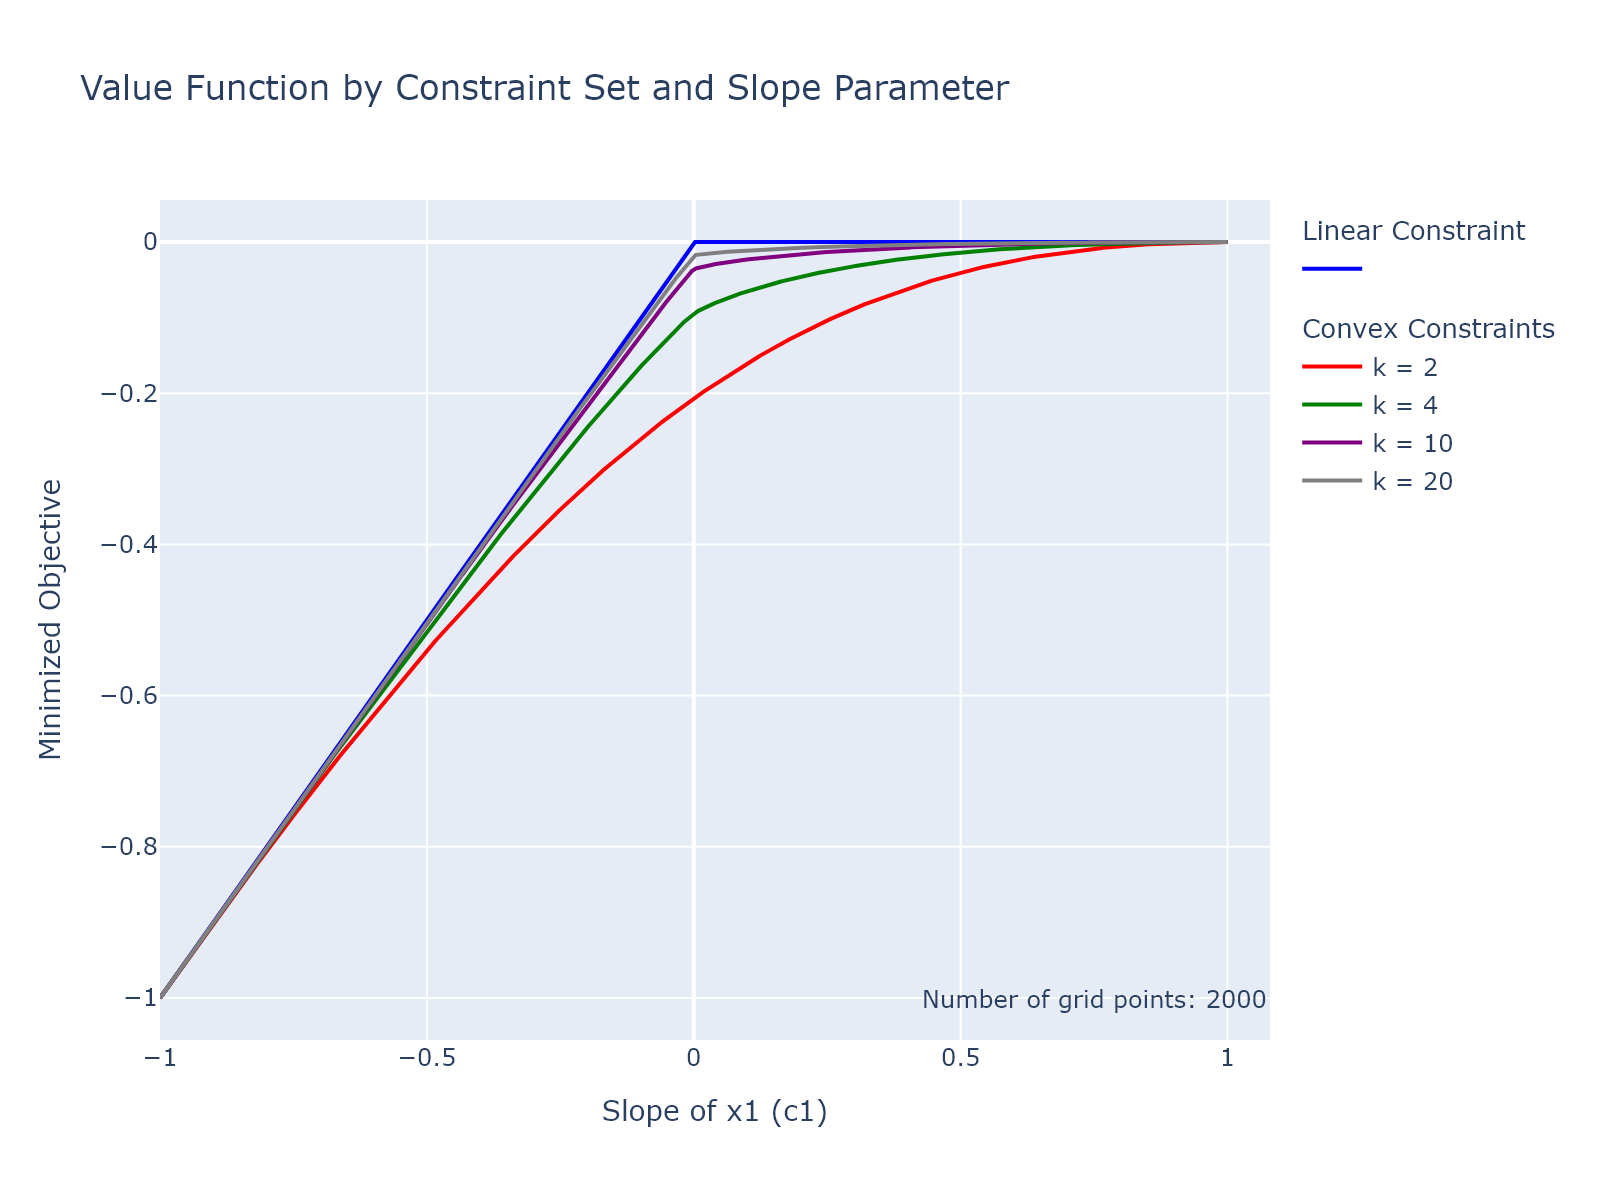
\includegraphics[width=\textwidth]{../figures/relax/value_function_by_constraint_set_dim_2.png}
        \caption{Value Functions}\label{fig:convex_relax_value}
      \end{subfigure}
      \hfill
      \begin{subfigure}[b]{0.49\textwidth}
        \centering
        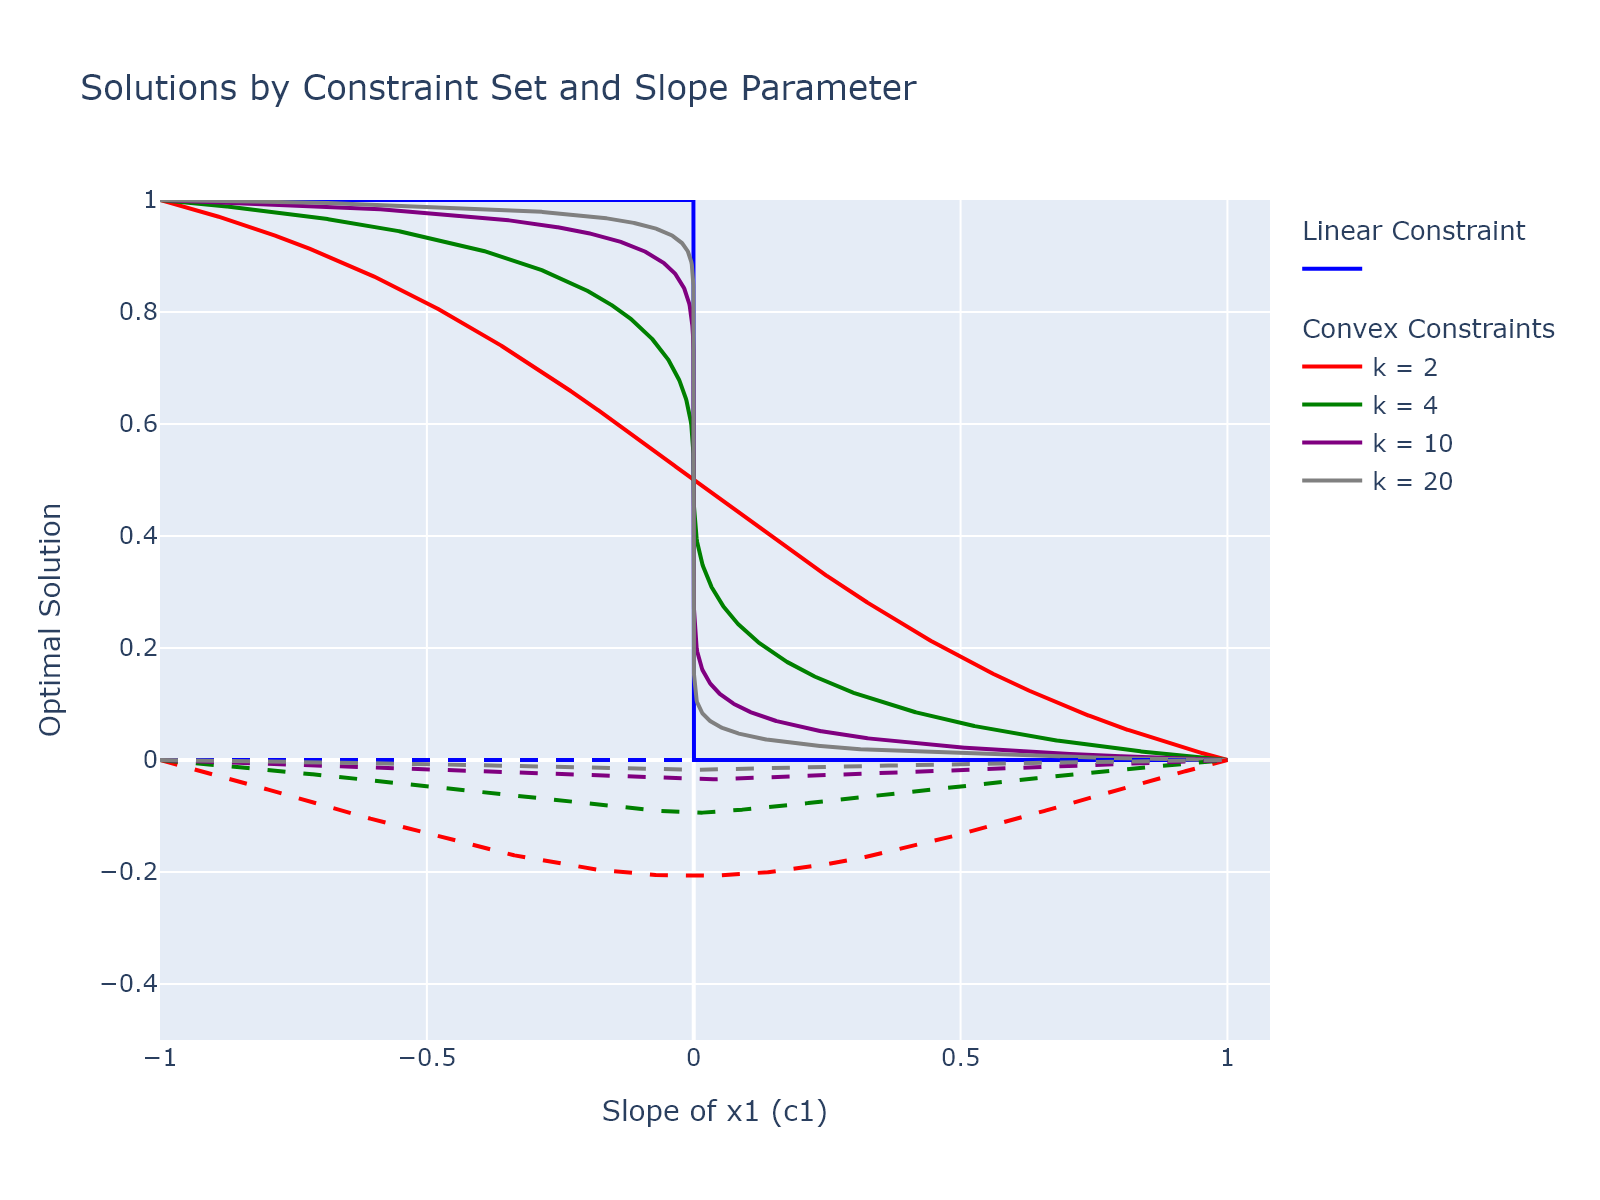
\includegraphics[width=\textwidth]{../figures/relax/solutions_by_constraint_set_dim_2.png}
        \caption{Solutions}\label{fig:convex_relax_solution}
      \end{subfigure}

      \begin{subfigure}[b]{0.49\textwidth}
        \centering
        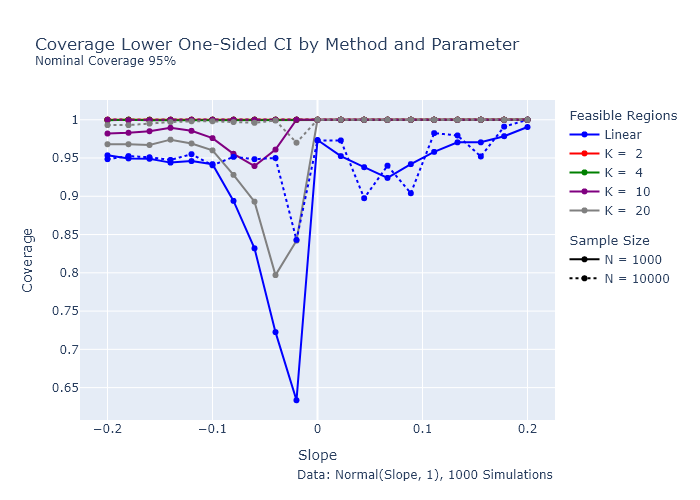
\includegraphics[width=\textwidth]{../figures/relax/covers_lower_one_sided_by_method.png}
        \caption{One-Sided CI:\@ Coverage}\label{fig:convex_relax_ci_coverage}
      \end{subfigure}
      \hfill
      \begin{subfigure}[b]{0.49\textwidth}
        \centering
        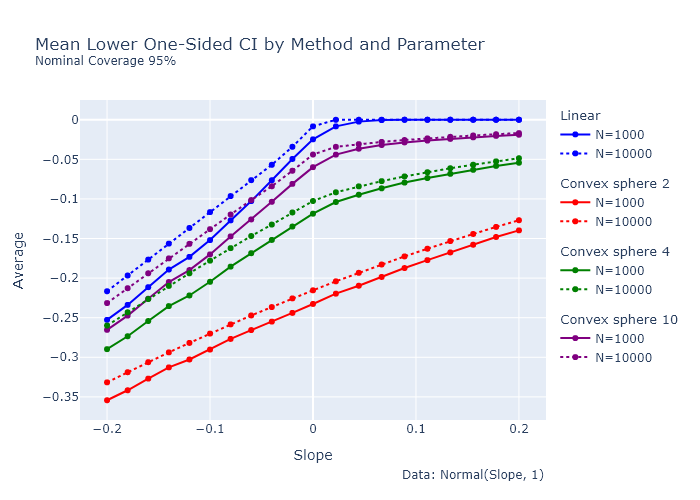
\includegraphics[width=\textwidth]{../figures/relax/lower_ci_one_sided_by_method.png}
      \caption{One-Sided CI:\@ Mean}\label{fig:convex_relax_ci_mean}
  \end{subfigure}

\end{figure}

\subsection{Discussion}
The foregone illustration already points to several of the weaknesses of this approach, which will be discussed in the following.

\paragraph{Inference on the Approximation}
The essential idea is to provide a (slightly) conservative approximation, for which we can perform inference.
However, even in this two-dimensional case, whenever $c_2=0$, the value function will feature a kink.
When $c_2=0$, level curves of the objective are parallel to the $x_2$-axis.
If $c_1 > 0$, the point of tangency is at the boundary of the feasible region where $x_1$ is minimal, for $c_1 < 0$ at the boundary where $x_1$ is maximal.
These points occur at $x_2=0.5$.
Call these values $x_1^{\min}, x_1^{\max}$.
The value function is then given by $I\{c_1 \leq 0\} c_1 x_1^{\max} + I\{c_1 > 0\} c_1 x_1^{\min} < 0$.
Since $x_1^{\max} > |x_1^{\min}|$, the value function has a kink at $c_0$.
However, $c = 0$ should be excluded in most applications of interest.
Specifically, in our case, choosing a relevant target parameter should always ensure that $c$ is bounded away from zero.
In the simple example, this would only include the situation where both $p(0) \approx p(1)$ and $\overline{u} \approx 0$, but the latter is chosen by the researcher.

More generally,~\cite{shapiro1991asymptotic} Section 3 discusses several adjustments of the delta method for inference on the objective function in mathematical programming.
In particular, Theorem 3.1 provides the Hadamard directional derivative for the value function when only the objective has a stochastic component.
Further, it is noted that if the solution is unique, then this derivative is linear and the value function is hence \textit{fully} differentiable.
In that case, as expected, if the asymptotic distribution of the stochastic part of the value function is normal, so is the optimal value.
This would be the case in our example since $\sqrt{N}(\hat{c_1} - c_1) \to_d N(0,\sigma^2)$ then $\sqrt{N}(\hat{\phi}_n - \phi_0) \to_d N(0,\sigma^2)$.
For the result see Theorem 3.3 and the preceding discussion.
If we exclude $c=0$ from the parameter space, then the example problem above has a unique solution everywhere and hence the above theorem applies.
\footnote{We also require $\mathcal{A}$ to be compact, which is true since it is closed and bounded.
Further, (a) $g(x, \omega) = \hat{c_1}x_0$ is measurable for all $x \in \mathcal{A}$, (b) it has a finite second moment, and (c) there exists a dominating function since $g$ is linear in $x$.}
[TODO Is this so relevant here?]

If all or some of the constraints are unknown, equivalent asymptotic results can be derived in settings with convex inequality constraints.
See Theorems 3.4 for the directional derivative and Theorem 3.5 for the asymptotic distribution.
Again, for a unique solution, this distribution is normal, with variance equal to the variance of the Lagrangian evaluated at the optimal solution.
Hence, this takes into account uncertainty both in the objective function and the constraints.
Since the $l_1$ norm in the MTE estimation linear program is convex, replacing the box constraint by a convex relaxation would give such a program.

\paragraph{Choosing $\mathcal{A}$}
Figure~\ref{fig:convex_relax_solution} shows a potential problem with norm-based relaxations $\mathcal{A}$:
The solution is too far away from the linear solution away from the kink, but changes too quickly at the kink, especially for high $k$.

Even given a set $\mathcal{A}$ that has desirable properties, the main challenge is motivating the tuning parameter, e.g. $k$ above.
While asymptotic theory probably puts some requirements on the rate of convergence to points of non-differentiability (probably slow ``enough'' relative to estimation rates), it is unclear how to motivate this choice in finite sample.
How useful such an approach would be in practice hinges on the ability to motivate a tuning parameter choice, which, for example, is the main problem with subsampling.
One potential source of information could be solving the estimation problem at hand under increasing relaxations as well as comparing the degree of conservativeness to an initial (biased) bootstrap estimate of the standard error.

\paragraph{Optimization Problem}
Linear programs can be solved reliably and fast to global optimally, in particular in many relevant applications of the MTE method.
The nonlinear problem resulting from the convex relaxation is, however, more difficult to solve in general.
In particular, numerical instability can be a concern when $\mathcal{A}$ is defined by a large $k$.
Also setting up the problem correctly takes more care and different optimizers with different strategies have to be employed on a case-by-case basis.

To illustrate these difficulties, I consider one of the MTE problems studied in Section~\ref{sec:simple_example}, namely a Bernstein polynomial of degree 11 with no shape restrictions, implying $2*12=24$ parameters.
Four equality constraints for the point-identified estimands reduce the number of free parameters to $20$; reparameterization is performed in the background by \textit{optimagic}.
The unit box $[0,1]^{24}$ is the only other constraint and I again relax it by the recentered norms of degree $k$.
Appendix Figure [TODO] plots the resulting approximations to the lower bound.
Sub-figure (a) provides approximations for varying $k$, while sub-figure (b) considers solutions for $k=20$ with multiple algorithms.
Notably, to get a close enough approximation, $k=20$ or $k=40$ is required. However, the solution is visibly unstable, pointing to optimization issues.
Further, different optimization routines result in partly vastly different solutions, pointing to convergence issues.
This is not meant to show, that this approach is generally not viable for higher dimensional problems, but to point out that several additional optimization difficulties are introduced by relaxing the constraint.


\section{Conclusion}

\paragraph{Extensions}
\begin{itemize}
  \item (More) Sharp identified set, see~\cite{marx2024sharp} (and another paper?).
  \item More complicated selection model, see~\cite{dutz2021selection}.
  \item Other inference approaches: Projection approach in~\cite{bei2023inference}.
\end{itemize}

\clearpage
\newpage


\bibliographystyle{abbrvnat}
\bibliography{refs.bib}

% \printbibliography % use this for biblatex

\appendix
\counterwithin{figure}{section}


\section{Binary IV Model: Solutions}
\subsection{Identified Estimands: Complier LATE}
\begin{figure}

  \caption{Identified Sets for the Binary-IV-Bernstein: Shape Restrictions}\label{app_fig:id_set_binary_iv_bernstein_shape_restrictions}

  \centering
  \begin{subfigure}[b]{0.49\textwidth}
      \centering
      \includegraphics[width=\textwidth]{../../bld/figures/binary_iv/id_bernstein_2_monotone_response_late.png}
      \caption{Positive Treatment Response ($k=2$)}\label{app_fig:id_set_binary_iv_bernstein_k_2_monotone_response}
  \end{subfigure}
  \hfill
  \begin{subfigure}[b]{0.49\textwidth}
      \centering
      \includegraphics[width=\textwidth]{../../bld/figures/binary_iv/id_bernstein_11_monotone_response_late.png}
      \caption{Positive Treatment Response ($k=11$)}\label{app_fig:id_set_binary_iv_bernstein_k_11_monotone_response}
  \end{subfigure}

  \begin{subfigure}[b]{0.49\textwidth}
      \centering
      \includegraphics[width=\textwidth]{../../bld/figures/binary_iv/id_bernstein_2_mte_monotone_late.png}
      \caption{Decreasing MTE ($k=2$)}\label{app_fig:id_set_binary_iv_bernstein_k_2_mte_monotone}
  \end{subfigure}
  \hfill
  \begin{subfigure}[b]{0.49\textwidth}
      \centering
      \includegraphics[width=\textwidth]{../../bld/figures/binary_iv/id_bernstein_11_mte_monotone_late.png}
      \caption{Decreasing MTE ($k=11$)}\label{app_fig:id_set_binary_iv_bernstein_k_11_mte_monotone}
  \end{subfigure}


\end{figure}

\subsection{Identified Estimands: Sharp Identified Set}
\begin{figure}

  \caption{Identified Sets for the Binary-IV-Bernstein: Shape Restrictions}\label{app_fig:id_set_binary_iv_bernstein_shape_restrictions_sharp}

  \centering
  \begin{subfigure}[b]{0.49\textwidth}
      \centering
      \includegraphics[width=\textwidth]{../../bld/figures/binary_iv/id_bernstein_2_monotone_response_sharp.png}
      \caption{Positive Treatment Response ($k=2$)}\label{app_fig:id_set_binary_iv_bernstein_k_2_monotone_response_sharp}
  \end{subfigure}
  \hfill
  \begin{subfigure}[b]{0.49\textwidth}
      \centering
      \includegraphics[width=\textwidth]{../../bld/figures/binary_iv/id_bernstein_11_monotone_response_sharp.png}
      \caption{Positive Treatment Response ($k=11$)}\label{app_fig:id_set_binary_iv_bernstein_k_11_monotone_response_sharp}
  \end{subfigure}

  \begin{subfigure}[b]{0.49\textwidth}
      \centering
      \includegraphics[width=\textwidth]{../../bld/figures/binary_iv/id_bernstein_2_mte_monotone_sharp.png}
      \caption{Decreasing MTE ($k=2$)}\label{app_fig:id_set_binary_iv_bernstein_k_2_mte_monotone_sharp}
  \end{subfigure}
  \hfill
  \begin{subfigure}[b]{0.49\textwidth}
      \centering
      \includegraphics[width=\textwidth]{../../bld/figures/binary_iv/id_bernstein_11_mte_monotone_sharp.png}
      \caption{Decreasing MTE ($k=11$)}\label{app_fig:id_set_binary_iv_bernstein_k_11_mte_monotone_sharp}
  \end{subfigure}
\end{figure}

\clearpage
\newpage

\section{Additional Simulation Results}

\subsection{Coverage by Tolerance}

\clearpage
\newpage

\section{Linear Programs}\label{app_sec:linear_programs}
This section presents the exact formulation of the linear programs corresponding to how most solvers specify linear programs.
I illustrate the actual programs in the case of binary IV model with an identified complier LATE/IV slope coefficient.
[Add programs for sharp identified set?]

\subsection{Identification}

The program for the upper bound is formulated as follows in~\cite{mogstad2018using}:
\begin{align}
  \overline{\beta}^* \equiv \sup_{(\theta_0, \theta_1)\in\Theta} \sum_{k=1}^{K_0}\theta_{0k}\Gamma^*_0(b_{0k}) + \sum_{k=1}^{K_1}\theta_{1k}\Gamma^*_1(b_{1k}) \\
  \text{subject to} \qquad \sum_{k=1}^{K_0}\theta_{0k}\Gamma_{0s}(b_{0k}) + \sum_{k=1}^{K_1}\theta_{1k}\Gamma_{1s}(b_{1k}) = \beta_s \text{ for } s \in \mathcal{S}.
\end{align}

In words: We maximize the target parameter, where we maximize over a basis function approximation with coefficients in a set $\Theta$.
The first summation term corresponds to $m_0$, the second to $m_1$.
We can separately parametrize $m_0$ and $m_1$ as reflected by the potentially different number of basis coefficients $K_0$ and $K_1$.
$\Theta$ can implicitly incorporate other constraints, like shape restrictions on $m_0, m_1$ which will be made explicit below.
It will at least entail the restrictions that $m_0, m_1$ are bounded by the support of the outcome $Y$, which we take to be $[0,1]$ without loss of generality.

Explicitly stated in the second line are the restrictions that for each point-identified estimand $s\in\mathcal{S}$ the maximizers $(\theta_0, \theta_1)$ must recover the point-identified parameter.

\paragraph{Matrix Form}
Next, I explicitly define the matrices typically used to describe a linear program.
In the so-called \textit{standard form}, all linear programs are described by:
(1) A \textit{maximization} objective; (2) inequality constraints with upper bounds; (3) non-negativity constraints on the choice variables.
Hence, we have:

\begin{align}
  \max_x c'x \\
  \text{ subject to } Ax\leq b, x\geq0
\end{align}

To keep the notation lighter, I instead reformulate the program in terms of:
(1) A \textit{minimization} objective; (2) inequality constraints with upper bounds; (3) equality constraints; (4) lower and upper bounds on the choice variables.
In this case, the program is:

\begin{align}
  \min_x c'x \\
  \text{ subject to } A_{ub}x \leq b_{ub}, A_{eq} = b_{eq}, l\leq x\leq u.
\end{align}

This is, for example, how the linear program is inputted into the \texttt{SciPy} \texttt{linprog} solver.
The program can easily be transformed to standard form by: (1) taking the negative of the objective, (2) reformulating equalities as two inequalities, and (3) expressing variables without positivity constraints as differences of two non-negative variables.
\texttt{SciPy}, for example, performs these operations in addition to other pre-solve checks for potential simplifications in the background.
It then passes the standard form program to a solver and post-processes the result to a solution of the original problem.

For simplicity, in the following we take $K_0 = K_1 = K$. This is the case for nonparametric exact bounds using constant splines and also parametric cases there seems little reason to have different numbers of basis polynomials.
Further, it simplifies the formulation of shape restrictions.

The choice variables are the basis function coefficients
\begin{equation*}
  x =
  \begin{bmatrix}
     \theta_{01} & \cdots & \theta_{0K} & \theta_{11} & \cdots & \theta_{1K}
  \end{bmatrix}',
\end{equation*}
and the coefficients are the individual contributions to the target parameter
\begin{equation*}
  c =
  \begin{bmatrix}
     \Gamma_0^*(b_{01}) & \cdots & \Gamma_0^*(b_{0K}) & \Gamma_1^*(b_{11}) & \cdots & \Gamma_1^*(b_{1K})
  \end{bmatrix}'.
\end{equation*}
Both of these are vectors of length $2K$.

Next, we have an equality constraint for each point-identified estimand $s\in\mathcal{S}$.
\begin{equation*}
  a_{eq}^s =
  \begin{bmatrix}
     \Gamma_{0s}(b_{01}) & \cdots & \Gamma_{0s}(b_{0K}) & \Gamma_{1s}(b_{11}) & \cdots & \Gamma_{1s}(b_{1K})
  \end{bmatrix}.
\end{equation*}
Note that we changed the map from $\Gamma^*_d$ to $\Gamma_{ds}$. Stacking these row-vectors gives the equality constraint matrix:
\begin{equation*}
  A_{eq}^s =
  \begin{bmatrix}
    a_{eq}^1 \\
    \vdots \\
    a_{eq}^\mathcal{S} \\
  \end{bmatrix},
\end{equation*}
which is a matrix of dimension $(S\times 2K)$, where, for brevity, we denote the \textit{number} of identified estimands $|\mathcal{S}| = S$.
The constraint values are given by the point-identified estimands:
\begin{equation*}
  b_{eq} =
  \begin{bmatrix}
    \beta_1, \ldots, \beta_\mathcal{S}
  \end{bmatrix}'.
\end{equation*}


A set of restrictions to achieve a minimal degree of identification is $y_l \leq m_d \leq y_d$ for $d=0,1$ and $y_l, y_u$ the lower and upper bound of the support of $Y$.
Taking $y_l = 0, y_u=1$, for typical shape constraints --- constant splines or Bernstein polynomials --- this amounts to the restrictions $0\leq \theta_{dj} \leq 1$ for $d=0,1, j=1,\ldots,K$.
Hence, we have the restrictions
\begin{equation*}
  l = \mathbf{0} \leq x \leq \mathbf{1} = u,
\end{equation*}
where $l$ and $u$ are vectors of length $2K$ each.

Finally, a number of shape restrictions may be added in the form of inequality bounds $A_{ub} \leq b_{ub}$.
The following applies to constant splines and Bernstein polynomials, but might not hold for all possible types of basis functions.

\paragraph{MTR Monotonicity}
To enforce a \textit{decreasing} MTR function $m_d(u)$ for constant splines, it is immediate that $\theta_{d1} \geq \theta_{d2} \geq \cdots \geq \theta_{dK}$, given that the functions are ordered over the partition of $u$, which we always assume to be the case.
For Bernstein polynomials this also holds, since they obey a monotonicity property: Whenever the basis coefficients $\theta_{dk}$ are decreasing over $k$, so is the resulting Bernstein polynomial (and the same for increasing).

Hence, to enforce a decreasing MTR function for $d=0$ we add the following constraints:
% \begin{equation*}
%   A_{eq}^s =
%   \begin{bmatrix}
%     -1 & 1 & 0 & \cdots & 0 & 0\\
%     0 & -1 & 1 & \cdots & 0 & 0\\
%     \vdots & & & \vdots \\
%     0 & 0 & 0 & \cdots & -1 & 1\\
%   \end{bmatrix} + \mathbf{0}
% \end{equation*}

\begin{equation*}
  A_{ub} =
  \begin{bNiceArray}{ccccccc}
    -1 & 1 & 0 & \cdots & 0 & 0 & \Block{4-1}<\Large>{\mathbf{0}}\\
    0 & -1 & 1 & \cdots & 0 & 0\\
    \vdots & & & \vdots \\
    0 & 0 & 0 & \cdots & -1 & 1\\
  \end{bNiceArray} \leq \mathbf{0} = b_{ub}.
\end{equation*}
Here, the first block is of dimension $(K-1) \times K$ reflecting the inequalities on the basis functions for $m_0(u)$.
The second block are zeros of dimension $(K-1) \times K$ on the basis functions for $m_1(u)$.
To add a similar restriction on $m_1(u)$ we can switch the blocks.
To enforce \textit{increasing} MTR functions $A_{ub}$ above can be multiplied by $-1$ to flip the inequalities.
$b_{ub}$ has length $(K-1)$.

\paragraph{MTE Monotonicity}
To enforce a \textit{decreasing} MTE function (the difference $m_1(u) - m_0(u)$) we require
$\theta_{11} - \theta_{01} \geq \theta_{12} - \theta_{02} \geq \cdots \geq \theta_{1K} - \theta_{0K}$.
For both constant splines and Bernstein polynomials this is immediate, since the difference $m_1(u) - m_0(u)$ implies a set of basis functions with the above differences as coefficients, which, hence, obey the same monotonicity conditions.

\begin{equation*}
  A_{ub} =
  \begin{bmatrix}
    \ldots
  \end{bmatrix} \leq \mathbf{0} = b_{ub}
\end{equation*}

\paragraph{Monotone Treatment Response}
Monotone treatment response requires $m_1(u) - m_0(u) \geq 0$ (positive) or $m_1(u) - m_0(u) \leq 0$ (negative) for all $u$.
Hence, we require $\theta_{1j} - \theta_{0j} \geq 0$ for all $j=1,\ldots,K$ for positive responses and reversed for negative.
\begin{equation*}
  A_{ub} =
  \begin{bmatrix}
    \ldots
  \end{bmatrix} \leq \mathbf{0} = b_{ub}
\end{equation*}

\subsection{Estimation}
Estimation is more involved and features solving two linear programs.
~\cite{mogstad2018using} propose a two-step estimator.
The reason is, that in sample we might not always expect all equality constraints for the identified estimands to be satisfied.
To allow for some sampling uncertainty, in a first step we compute the minimal achievable deviations from all point-identified estimands (as measured by the $l_1$ norm).
In the second step, we then restrict the set of allowed MTR functions to maximize over to those achieving this minimal deviation plus some tolerance.
In this way, the program always has a solution, meaning our estimators always exists.

This approach is stated in equation (27) of~\cite{mogstad2018using}:
\begin{align}
  & \hat{\overline{\beta}^*} \equiv \sup_{m\in \mathcal{M}}\hat{\Gamma}^*(m) \\
  & \text{ subject to } \sum_{s\in\mathcal{S}}|\hat{\Gamma}_s(m) - \hat{\beta}_s| \leq \inf_{m'\in \mathcal{M}} \sum_{s\in\mathcal{S}}|\hat{\Gamma}_s(m') - \hat{\beta}_s| + \kappa_n
\end{align}

Note we have a single constraint for the $l_1$ norm.
The $\inf$ on the right-hand side is the first-step linear program, and we allow for tolerance $\kappa_n$ to enlarge the set of possible solutions.

\subsubsection{First Step Linear Program}
The first step program is given by
\begin{equation*}
  \inf_{m'\in \mathcal{M}} \sum_{s\in\mathcal{S}}|\hat{\Gamma}_s(m') - \hat{\beta}_s|
\end{equation*}

We again rewrite it in the matrix form stated above.
Note that $\mathcal{M}$ again implicitly encodes any bounds and other shape restrictions on the MTR functions.
Further, as pointed out in~\cite{mogstad2018using}, we need to introduce dummy variables to mimic the absolute values in the objective.

\paragraph{Absolute Values in the Objective}
With $S = 1$, that is a single point-identified estimand, we have an objective of the following form:
\begin{equation*}
  \inf_m |X_1|,
\end{equation*}

where $X_1 = \hat{\Gamma}_1(m) - \hat{\beta}_1$.
We now add a dummy variable $X_1'$ and two constraints to the model:
\begin{align*}
  X_1 \leq X_1', \\
  -X_1 \leq X_1'.
\end{align*}
In the objective we replace the absolute value with the dummy:
\begin{equation*}
  \inf X_1'.
\end{equation*}
By going through all possible cases ($X_1=0, X_1<0, X_1>0$) it is easy to show,
that $X_1'$ will behave like $|X_1|$.

Having $|S|>1$ is then simply a matter of adding another dummy and two constraints per point-identified estimand.

Plugging in the original expression for $X_1$ we get
\begin{align*}
  \inf X_1' \\
  \text{ subject to }\\
  \hat{\Gamma}_1(m) - \hat{\beta}_1 \leq X_1', \\
  -(\hat{\Gamma}_1(m) - \hat{\beta}_1) \leq X_1',
\end{align*}
where minimization is now over the basis coefficients (appearing in the constraints) and the dummy variables (appearing in the objective).
Hence, we now have $2K + S$ choice variables.

The vector of choice variables is given by
\begin{equation*}
  x^{fs} =
  \begin{bmatrix}
     \theta_{01} & \cdots & \theta_{0K} & \theta_{11} & \cdots & \theta_{1K} & X_1' & \cdots & X_{S}
  \end{bmatrix}',
\end{equation*}
with corresponding coefficients

\begin{equation*}
  c^{fs} =
  \begin{bmatrix}
     \mathbf{0}', \mathbf{0}', \mathbf{1}'
  \end{bmatrix}',
\end{equation*}
where the zeros on the basis functions are of length $K$ each and the $1$ on the dummies of length $S$.
Both of these are vectors of length $2K + S$.


To encode the first type of inequality for all $S$ we get the following inequality constraint matrix:
\begin{equation*}
  A_{ub, 1}^{fs} =
  \begin{bmatrix}
    \hat{\Gamma}_{01}(b_{01}) & \cdots & \hat{\Gamma}_{01}(b_{0K}) & \hat{\Gamma}_{11}(b_{11}) & \cdots & \hat{\Gamma}_{11}(b_{1K}) & -1 & 0 & \cdots & 0 \\
    \vdots & & \vdots & \vdots &  & \vdots & \\
    \hat{\Gamma}_{0S}(b_{01}) & \cdots & \hat{\Gamma}_{0S}(b_{0K}) & \hat{\Gamma}_{1S}(b_{11}) & \cdots & \hat{\Gamma}_{1S}(b_{1K}) & 0 & 0 & \cdots & -1 \\
  \end{bmatrix}
\end{equation*}
which is of dimension $S\times (2K + S)$. The upper bounds are the estimated point-identified estimands:

\begin{equation*}
  b_{ub, 1}^{fs} =
  \begin{bmatrix}
    \hat{\beta}_1 & \cdots & \hat{\beta}_S
  \end{bmatrix}'.
\end{equation*}

To encode the second type of constraint we multiply the first $2K$ columns of $A_{ub, 1}^{fs}$ as well as the upper bounds by $-1$.

In the first step program, $c$ is a constant, while $A_{ub}^{fs}$ and $b_{ub}^{fs}$ need to be estimated from the data.

\subsubsection{Second Step Linear Program}
Denote the minimal deviation from the first step program, that is the value function, by $\mu$ (or $\hat{\mu}$, to emphasize the dependence on the data).

The choice variables in the second-step program are again only the basis function coefficients:
\begin{equation*}
  x^{ss} =
  \begin{bmatrix}
     \theta_{01} & \cdots & \theta_{0K} & \theta_{11} & \cdots & \theta_{1K} & X_1' & \cdots & X_S'
  \end{bmatrix}',
\end{equation*}
and the coefficients are the estimated individual contributions to the target parameter
\begin{equation*}
  c^{ss} =
  \begin{bmatrix}
     \hat{\Gamma}_0^*(b_{01}) & \cdots & \hat{\Gamma}_0^*(b_{0K}) & \hat{\Gamma}_1^*(b_{11}) & \cdots & \hat{\Gamma}_1^*(b_{1K}) & \mathbf{0}
  \end{bmatrix}'.
\end{equation*}
Both of these are vectors of length $2K + S$.

Note that the problem again features the $l_1$ norm, this time in the constraints.
Because we have a sum over multiple absolute values, we again introduce a dummy variable and two constraints that behaves like the absolute value for each point-identified estimand.
The only difference to the first-step constraint matrix is then the additional presence of the (relaxed) constraint on the $l_1$ norm:

\begin{equation*}
  a_{ub}^{ss, 1} = \begin{bmatrix}
    \mathbf{0} & \mathbf{1}
  \end{bmatrix}
  \leq \hat{\mu} + \kappa_n.
\end{equation*}
Here the first vector of zeros is of length $2K$ (the basis functions) and the vector of ones of length $S$ (the dummy variables).

The full second-step upper bound matrix is then given by
\begin{equation*}
  A_{ub}^{ss} = \begin{bmatrix}
    a_{ub}^{ss, 1} \\
    \mathbf{A_{ub,1}^{fs}} \\
    \mathbf{A_{ub,2}^{fs}} \\
  \end{bmatrix}
  \leq
  \begin{bmatrix}
    \hat{\mu} + \kappa_n \\
    \mathbf{\hat{\beta}} \\
    - \mathbf{\hat{\beta}} \\
  \end{bmatrix}
  = b_{ub}^{ss}.
\end{equation*}

The full program is then
\begin{align}
  & \min_x \hat{c}^{ss'}x^{ss} \text{ subject to }\\
  & \hat{A}_{ub}^{ss} \leq \hat{b}_{ub}^{ss} \\
  & \mathbf{0} \leq x^{ss} \leq \mathbf{1},
\end{align}
where $\hat{\cdot}$ is used to emphasize, which parts of the problem are estimated from the data.

\subsubsection{Shape Constraints}
Shape constraints need to be added to both the first and second step program.
All shape constraints are similar to the identification part, except for additional zero columns in $A_{ub}$ in the first step program due to the dummy variables.
In particular, all of these constraints are non-random.


% \subsection{Illustration: Binary IV Model with Point-Identified LATE}


% \subsection{Illustration: Binary IV Model with Sharp Identified Set}


\end{document}
